\documentclass{article}


\usepackage{PRIMEarxiv}

\usepackage[utf8]{inputenc} % allow utf-8 input
\usepackage[T1]{fontenc}    % use 8-bit T1 fonts
\usepackage[linkbordercolor={1 0 0}]{hyperref}%
\usepackage{multirow}
\usepackage{adjustbox}
\usepackage{url}            % simple URL typesetting
\usepackage{makecell}
\usepackage{booktabs}       % professional-quality tables
\usepackage{amsfonts}       % blackboard math symbols
\usepackage{nicefrac}       % compact symbols for 1/2, etc.
\usepackage{microtype}      % microtypography
\usepackage{lipsum}
\usepackage{fancyhdr}       % header
\usepackage{graphicx}       % graphics
\graphicspath{{media/}}     % organize your images and other figures under media/ folder
\usepackage{xcolor}
\usepackage{float}
\usepackage{amsmath}
\usepackage{dsfont}
\usepackage[french]{babel}
\usepackage{algorithm}
\usepackage{algorithmicx}
\usepackage[noend]{algpseudocode}
\usepackage{titlesec}
\renewcommand{\algorithmicrequire}{\textbf{Entrées:}}
\renewcommand{\algorithmicensure}{\textbf{Sortie:}}
\renewcommand{\algorithmicend}{\textbf{Fin}}
\renewcommand{\algorithmicif}{\textbf{Si}}
\renewcommand{\algorithmicthen}{\textbf{Alors}}
\renewcommand{\algorithmicelse}{\textbf{Sinon}}
\renewcommand{\algorithmicfor}{\textbf{Pour}}
\renewcommand{\algorithmicforall}{\textbf{Pour chaque}}
\renewcommand{\algorithmicdo}{\textbf{Faire}}
\renewcommand{\algorithmicwhile}{\textbf{Tant que}}
\renewcommand{\algorithmicreturn}{\textbf{Retourner}}
\renewcommand{\algorithmicprocedure}{\textbf{Procédure}}
\renewcommand{\algorithmicendprocedure}{\textbf{Fin procédure}}
\renewcommand{\algorithmicand}{\textbf{Et}}
\renewcommand{\algorithmicor}{\textbf{Ou}}



\titlespacing{\section}{0cm}{0.7cm}{0.3cm}
\titlespacing{\subsection}{0cm}{0.45cm}{0.2cm}

\RequirePackage{xcolor}

\newcommand{\cfootnote}[2][black]{%
    {\color{#1}\footnote{#2}}%
}

% Define the hyperlink color


%Header
\pagestyle{fancy}
\renewcommand{\headrulewidth}{0.4pt}% Default \headrulewidth is 0.4pt

% Update your Headers here
\fancyhead[RO,LE]{État de l'Art YOLO}
% \fancyhead[RE]{Firstauthor and Secondauthor} % Firstauthor et al. if more than 2 - must use \documentclass[twoside]{article}



  
%% Title
\title{État de l'Art YOLO : De YOLOv1 à YOLOv8
%%%% Cite as
%%%% Update your official citation here when published 
}

\author{
  MARZOUG Ayoub \\
  Data Engineering (DE) \\
  INPT \\
  Rabat\\
  \texttt{marzoug.ayoub@inemail.ine.inpt.ma} \\
  %% examples of more authors
   \And
  FEKRI Mohammed \\
  Mathématiques, Informatique et Réseaux \\
  INPT \\
  Rabat\\
  \texttt{fekri@inpt.ac.ma} \\
  %% \AND
  %% Coauthor \\
  %% Affiliation \\
  %% Address \\
  %% \texttt{email} \\
  %% \And
  %% Coauthor \\
  %% Affiliation \\
  %% Address \\
  %% \texttt{email} \\
  %% \And
  %% Coauthor \\
  %% Affiliation \\
  %% Address \\
  %% \texttt{email} \\
}



\begin{document}
\maketitle

\begin{center}
\text{Mai 19, 2023} 
\end{center}

\vspace{1cm}

\begin{abstract}
\vspace{0.8cm}

YOLO has become a central real-time object detection system for robotics, driverless cars, and video monitoring applications. We present a comprehensive analysis of YOLO’s evolution, examining the innovations and contributions in each iteration from the original YOLO to YOLOv8. We start by describing the standard metrics and postprocessing; then, we discuss the major changes in network architecture and training tricks for each model. Finally, we summarize the essential lessons from YOLO’s development and provide a perspective on its future, highlighting potential research directions to enhance real-time object detection systems.
\end{abstract}

\vspace{0.5cm}

% keywords can be removed
\keywords{YOLO \and Object detection \and Deep Learning \and Computer Vision}

\vspace{0.5cm}

\section{Préambule}
Ce document s’inscrit dans le sillage des projets exigibles au cours de la formation en ingénierie des données au sein de l’institut national des postes \& télécommunications (INPT), et consiste en la réalisation d'un panorama synthétique et organisé des travaux et publications majeures existants en rapport avec la technologie de détection d'objets YOLO, ainsi qu'un aperçu sur son développement et ses cas d’usage. Il marque le dénouement du mini-projet bibliographie et initiation à la recherche encadré par Mr. FEKRI Mohammed à qui je témoigne une profonde déférence, et à l’honorable examen duquel je laisse cet ouvrage en souhaitant qu’il réponde à ses propres souhaits, ainsi qu’aux espérances et à l’attente de ses lecteurs. Il va de soi qu’il ne porte aucune responsabilité pour les quelques débordements auxquels j’ai pu me laisser aller ni pour les quelques fautes\cfootnote[black]{Dont le nombre suit une loi de Poisson.} que l’on ne manquera pas de trouver dans cette édition\cfootnote[black]{Remerciements anticipés à tout lecteur qui m’aidera à réduire le paramètre de ladite loi.}.


\section{Introduction}

La détection en temps réel d'objets s'est imposée comme un composant crucial dans de nombreuses applications, couvrant divers domaines tels que les véhicules autonomes, la robotique, la vidéo-surveillance et la réalité augmentée. Parmi les différents algorithmes de détection d'objets, le framework YOLO (You Only Look Once) s'est distingué par son remarquable équilibre entre vitesse et précision, permettant l'identification rapide et fiable des objets au sein des images. Depuis sa création, la famille YOLO a évolué au fil des itérations, chacune s'appuyant sur les versions précédentes pour pallier les limitations et améliorer les performances (voir Figure \ref{fig:time}). Ce document vise à fournir une revue complète du développement du framework YOLO, depuis le YOLOv1 original jusqu'au dernier YOLOv8, en élucidant les innovations clés, les différences et les améliorations apportées à chaque version.
\vspace{0.2cm}\\
Le document commence par explorer les concepts fondamentaux et l'architecture du modèle YOLO original, qui a préparé le terrain pour les avancées ultérieures de la famille. Ensuite, on se penche sur les raffinements et les optimisations introduits dans chaque version, de YOLOv2 à YOLOv8. Ces améliorations comprennent divers aspects tels que la conception du réseau de neurones, les variations de la fonction de perte, les adaptations de la boîte d'ancrage et la mise à l'échelle de la résolution en  entrée. En examinant ces développements, on cherche à offrir une compréhension systémique de l'évolution du framework YOLO et de ses implications sur la détection d'objets.
\vspace{0.2cm}\\
Outre l'examen des avancées spécifiques de chaque version de YOLO, le document met en évidence les compromis entre la vitesse et la précision qui ont émergé tout au long du développement du framework. D'où l'importance de tenir compte du contexte et des exigences d'applications spécifiques lors de la sélection du modèle YOLO le plus idoine. Enfin, on envisage les orientations futures de la technique YOLO, en évoquant les pistes potentielles de recherche et de développement qui façonneront les progrès en cours des systèmes de détection d'objets en temps réel.

\begin{figure}[H]
    \centering
    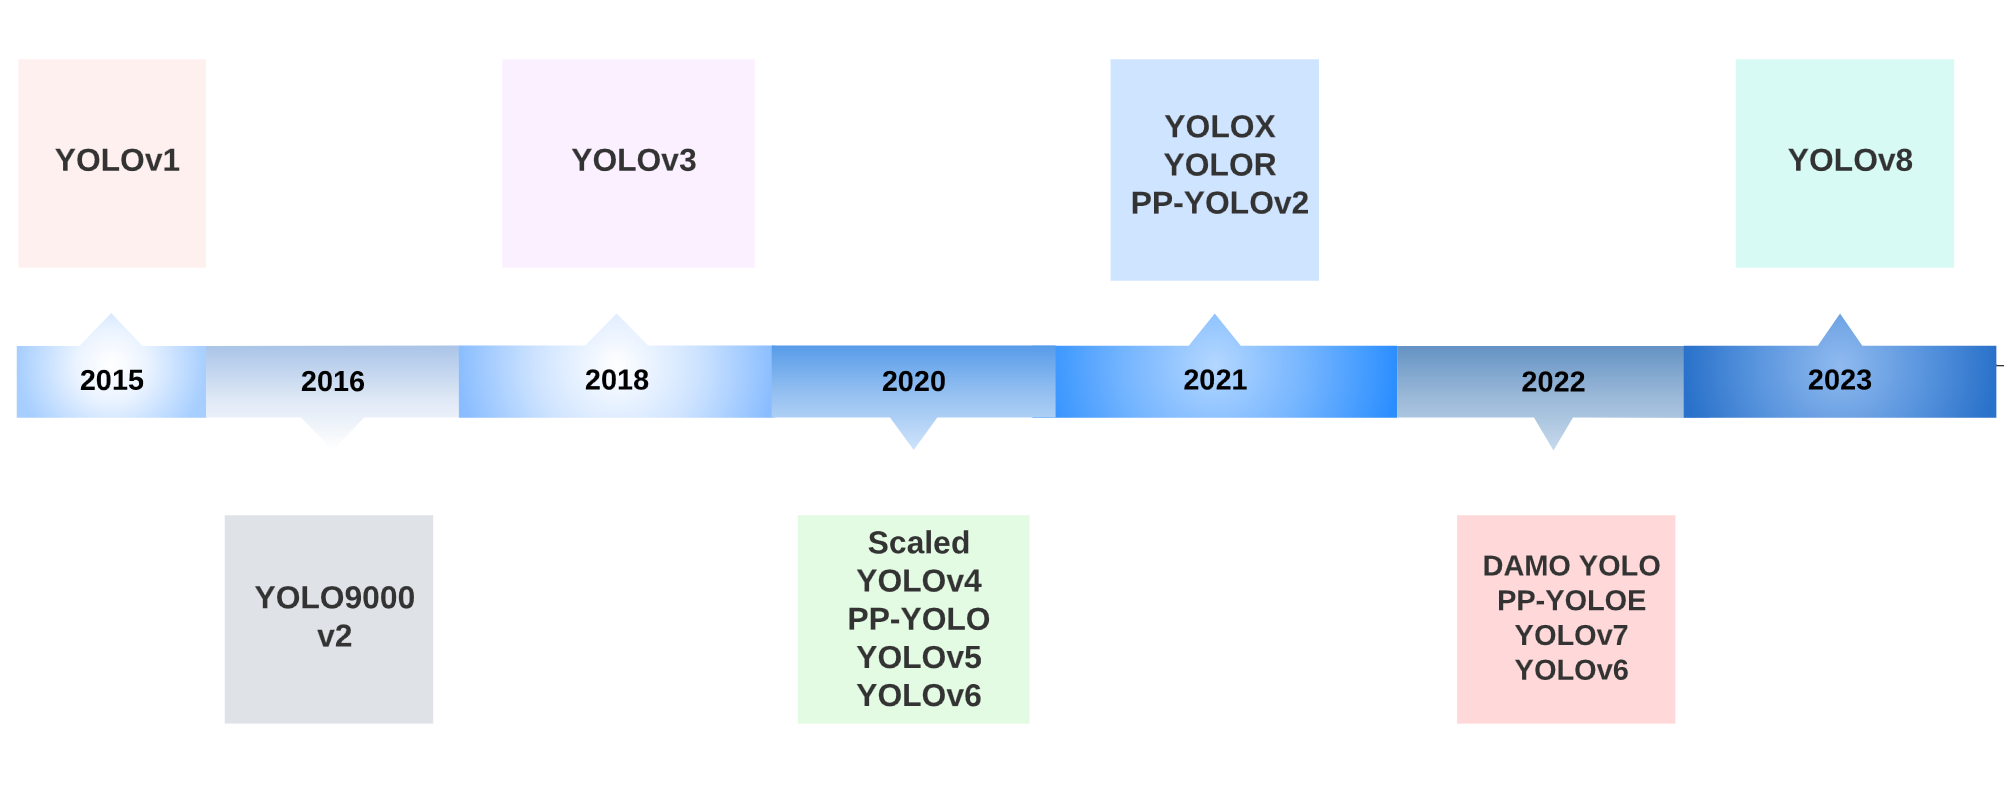
\includegraphics[scale=0.22]{Figures/timeline.png}
    \caption{Chronologie des versions YOLO}
    \label{fig:time}
\end{figure}
\vspace{0.5cm}


\section{Applications de YOLO}

Les capacités de détection d'objets en temps réel de YOLO se sont révélées inestimables dans les systèmes de véhicules autonomes, permettant l'identification rapide et le suivi de divers objets tels que les véhicules, les piétons \cite{1,2}, les vélos et autres obstacles \cite{3, 4, 5, 6}. Ces capacités ont été appliquées dans de nombreux domaines, notamment la reconnaissance d'actions \cite{7} dans des séquences vidéo pour la surveillance \cite{8}, l'analyse sportive \cite{9} et l'interaction homme-machine \cite{10}.
\vspace{0.2cm}\\
Les modèles YOLO ont été utilisés en agriculture pour détecter et classer les cultures \cite{11, 12}, les ravageurs et les maladies \cite{13}, contribuant aux techniques d'agriculture de précision et à l'automatisation des processus agricoles. Ils ont également été adaptés aux tâches de détection faciale dans les domaines de la biométrie, de la sécurité et des systèmes de reconnaissance faciale \cite{14, 15}.
\vspace{0.2cm}\\
Dans le domaine médical, YOLO a été utilisé pour la détection du cancer \cite{16, 17}, la segmentation de la peau \cite{18} et l'identification de pilules \cite{19}, ce qui a permis d'améliorer la précision du diagnostic et l'efficacité des traitements. En télédétection, il a été utilisé pour la détection et la classification d'objets dans les images satellite et aériennes, contribuant à la cartographie de l'utilisation des terres, à la planification urbaine et à la surveillance de l'environnement \cite{20, 21, 22, 23}.
\vspace{0.2cm}\\
Les systèmes de sécurité ont intégré des modèles YOLO pour la surveillance en temps réel et l'analyse des flux vidéo, permettant la détection rapide d'activités suspectes \cite{24}, la distanciation sociale et la détection de masques faciaux \cite{25}. Les modèles ont également été appliqués à l'inspection de surface pour détecter les défauts et les anomalies, améliorant le contrôle qualité dans les processus de fabrication et de production \cite{26, 27, 28}.
\vspace{0.2cm}\\
Dans les applications de trafic, les modèles YOLO ont été utilisés pour des tâches telles que la détection de plaques d'immatriculation \cite{29} et la reconnaissance de panneaux de signalisation \cite{30}, contribuant au développement de systèmes de transport intelligents et de solutions de gestion du trafic. Ils ont été utilisés dans la détection et la surveillance de la faune pour identifier les espèces en voie de disparition pour la conservation de la biodiversité et la gestion des écosystèmes \cite{31}. Enfin, YOLO a été largement utilisé dans les applications robotiques \cite{32, 33} et la détection d'objets à partir de drones \cite{34, 35}.

\section{Métriques de Détection d'Objets \& Suppression non Maximale (NMS)}
La Précision Moyenne (Average Precision, AP), traditionnellement appelée Précision Moyenne Globale (Mean Average Precision, mAP), est la métrique couramment utilisée pour évaluer les performances des modèles de détection d'objets. Elle mesure la précision moyenne pour l'ensemble des catégories, fournissant une valeur unique pour comparer différents modèles. Le jeu de données COCO ne fait pas de distinction entre AP et mAP. Dans le reste de ce document, on désignera cette métrique par AP.
\vspace{0.2cm}\\
Dans YOLOv1 et YOLOv2, le jeu de données utilisé pour l'entraînement et les tests était PASCAL VOC 2007 et VOC 2012 \cite{36}. Néanmoins, à partir de YOLOv3, le jeu de données utilisé est Microsoft COCO (Common Objects in Context) \cite{37}. La façon de calculer l'AP diffère pour ces jeux de données. Les sections suivantes expliqueront la logique derrière l'AP et comment elle est calculée.
\subsection{Fonctionnement de l'AP}
La métrique AP est basée sur les métriques de précision-rappel, gérant plusieurs catégories d'objets et définissant une prédiction positive à l'aide de l'Intersection sur Union (IoU).
\vspace{0.2cm}\\
\textbf{Précision et Rappel} : La précision mesure l'exactitude des prédictions positives du modèle, tandis que le rappel mesure la proportion de cas réellement positifs que le modèle identifie correctement. Il y a souvent un compromis entre la précision et le rappel ; par exemple, augmenter le nombre d'objets détectés (augmentation du rappel) peut entraîner plus de faux positifs (baisse de la précision). Pour prendre en compte ce compromis, la métrique AP intègre la courbe de précision-rappel qui trace la précision en fonction du rappel pour différents seuils de confiance. Cette métrique fournit une évaluation équilibrée de la précision et du rappel en considérant l'aire sous la courbe de précision-rappel.
\vspace{0.2cm}\\
\textbf{Gestion de plusieurs catégories d'objets} : Les modèles de détection d'objets doivent identifier et localiser plusieurs catégories d'objets dans une image. La métrique AP aborde cela en calculant la précision moyenne (AP) de chaque catégorie séparément, puis en prenant la moyenne de ces AP pour toutes les catégories (c'est pourquoi on l'appelle également précision moyenne globale). Cette approche garantit que les performances du modèle sont évaluées pour chaque catégorie individuellement, fournissant une évaluation plus complète des performances globales du modèle.
\vspace{0.2cm}\\
\textbf{Intersection over Union} : La détection d'objets vise à localiser avec précision les objets dans les images en prédisant des boîtes englobantes. La métrique AP intègre la mesure de l'Intersection over Union (IoU) pour évaluer la qualité des boîtes englobantes prédites. L'IoU est le rapport entre la superficie d'intersection et la superficie d'union de la boîte englobante prédite et de la boîte englobante réelle (voir Figure \ref{fig:IoU}). Il mesure le chevauchement entre la boîte englobante réelle et la boîte englobante prédite. La référence COCO utilise plusieurs seuils d'IoU pour évaluer les performances du modèle à différents niveaux de précision de localisation.

\begin{figure}[htbp]
    \centering
    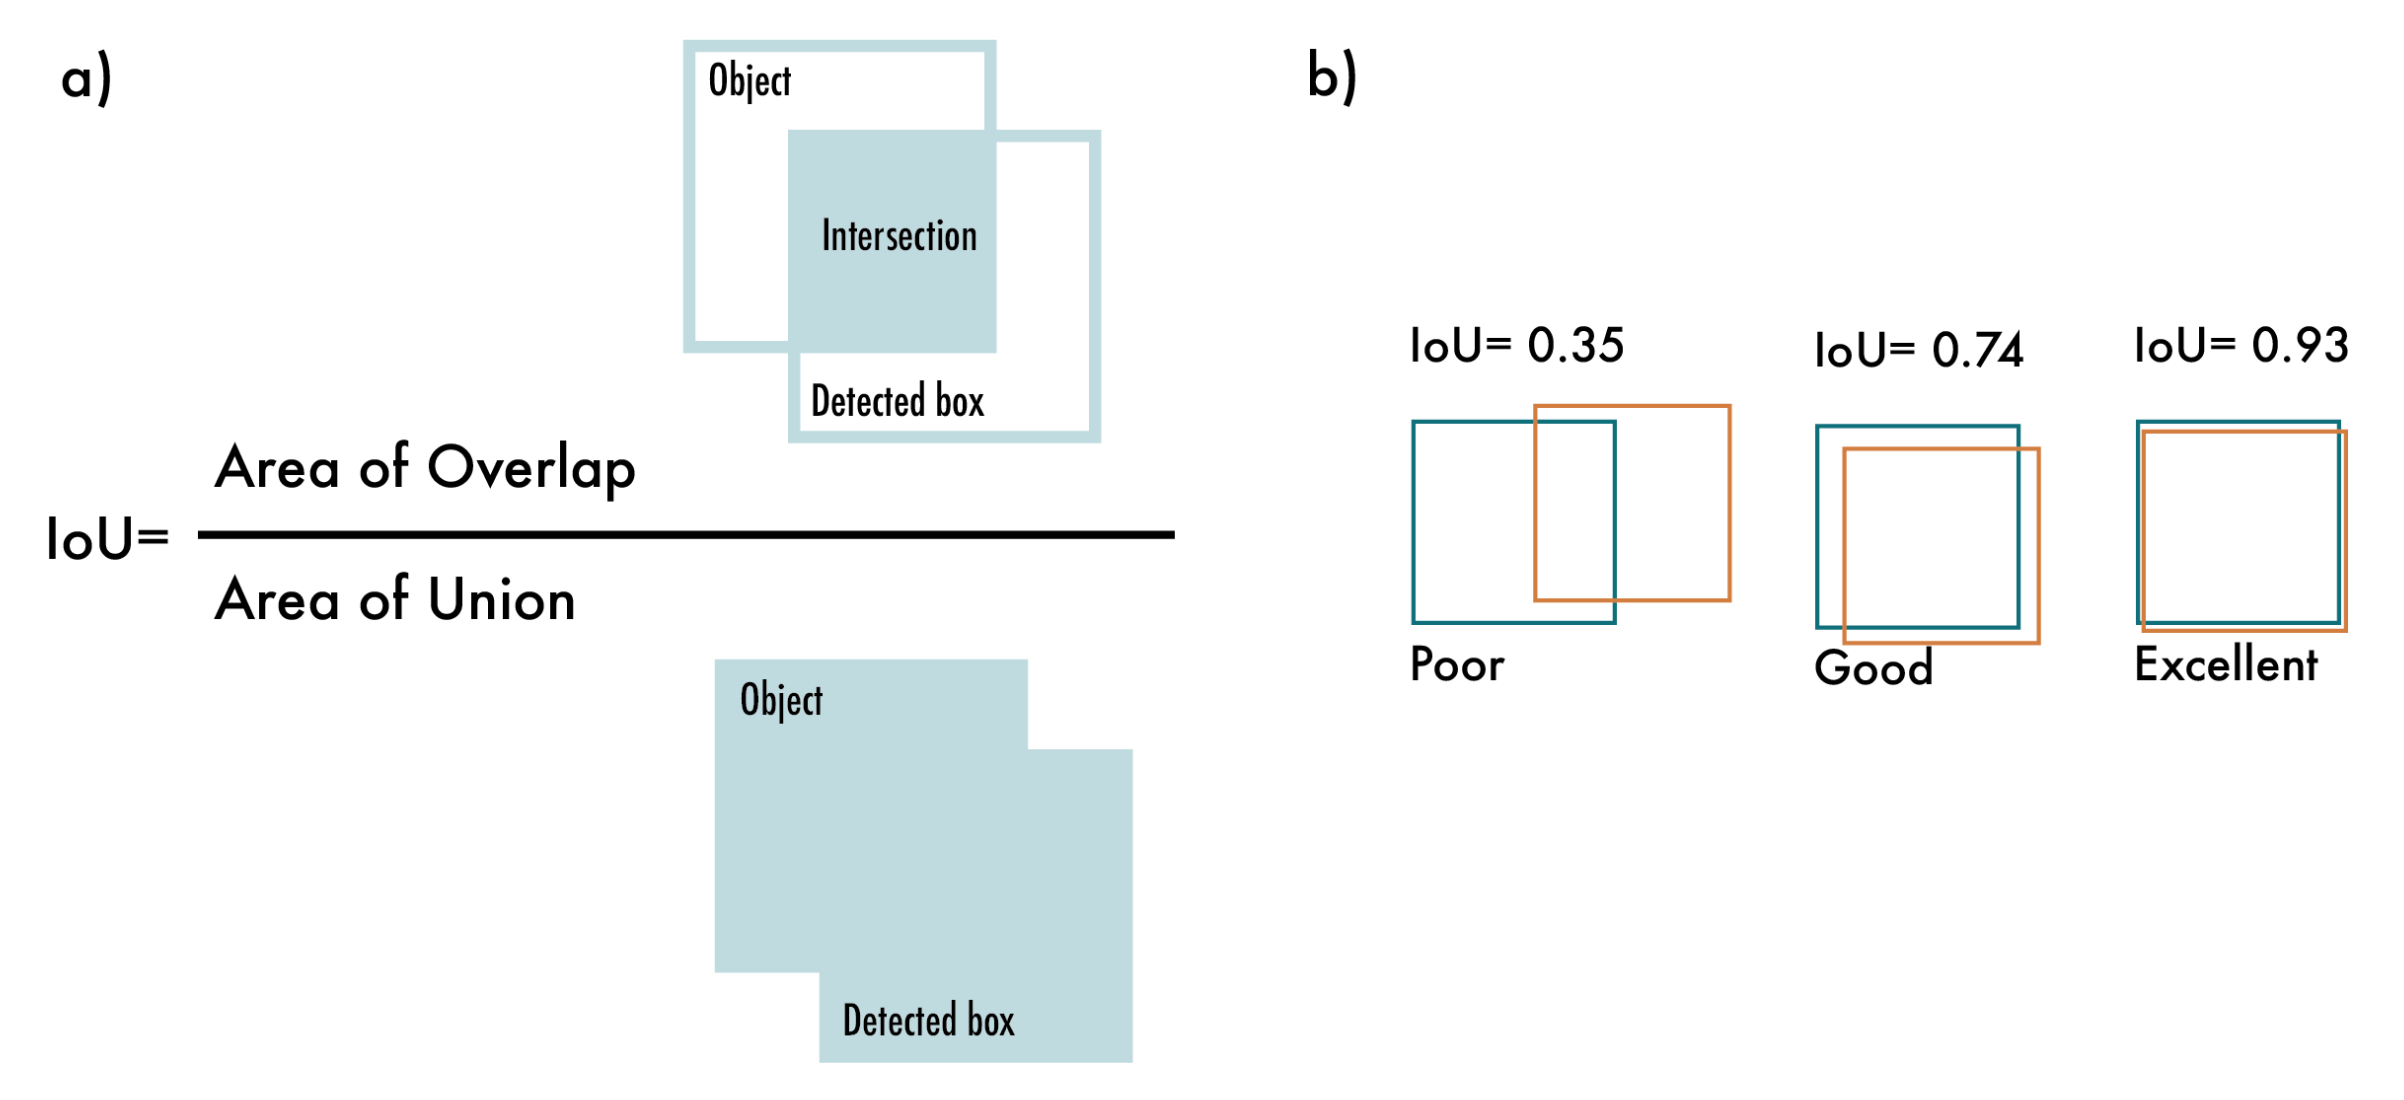
\includegraphics[scale=0.2]{Figures/IoU.png}
    \caption{Intersection over Union (IoU). a) L'IoU est calculé en divisant l'intersection des deux boîtes par l'union des boîtes ; b) exemples de trois valeurs différentes de l'IoU pour différents emplacements de boîtes.}
    \label{fig:IoU}
\end{figure}

\subsection{Calcul de l'AP}
L'AP est calculée différemment pour les jeux de données VOC et COCO. Dans cette section, on décrit comment elle est évaluée pour chaque dataset.

\subsection*{Dataset VOC}

Ce jeu de données comprend 20 catégories d'objets. Pour calculer l'AP pour VOC, on suit les étapes suivantes :
\begin{enumerate}
    \item Pour chaque catégorie, calculer la courbe précision-rappel en faisant varier le seuil de confiance des prédictions du modèle.
    \item Calculer la précision moyenne (AP) de chaque catégorie en utilisant un échantillonnage interpolé à 11 points de la courbe précision-rappel.
    \item Calculer la précision moyenne globale (AP) finale en prenant la moyenne des APs pour les 20 catégories.
\end{enumerate}

\subsection*{Dataset Microsoft COCO}

Ce jeu de données comprend 80 catégories d'objets et utilise une méthode plus complexe pour calculer l'AP. Au lieu d'utiliser une interpolation à 11 points, il utilise une interpolation à 101 points, c'est-à-dire qu'il calcule la précision pour 101 seuils de rappel de 0 à 1 avec des incréments de 0,01. De plus, l'AP est obtenu en moyennant sur plusieurs valeurs d'IoU au lieu d'une seule, à l'exception d'une métrique d'AP courante appelée {$AP_{50}$}, qui est l'AP pour un seuil d'IoU unique de 0,5. Les étapes pour calculer l'AP dans COCO sont les suivantes :
\begin{enumerate}
    \item Pour chaque catégorie, calculer la courbe précision-rappel en faisant varier le seuil de confiance des prédictions du modèle.
    \item Calculer la précision moyenne (AP) de chaque catégorie en utilisant 101 seuils de rappel.
    \item Calculer l'AP pour différents seuils d'Intersection sur Union (IoU), généralement de 0,5 à 0,95 avec un pas de 0,05. Un seuil d'IoU plus élevé nécessite une prédiction plus précise pour être considérée comme un vrai positif.
    \item Pour chaque seuil d'IoU, prendre la moyenne des AP pour les 80 catégories.
    \item Enfin, calculer l'AP global en faisant la moyenne des valeurs d'AP calculées à chaque seuil d'IoU.
\end{enumerate}
Les différences dans le calcul de l'AP rendent difficile la comparaison directe des performances des modèles de détection d'objets entre les deux jeux de données. La norme actuelle utilise l'AP COCO en raison de son évaluation plus détaillée de la performance d'un modèle à différents seuils d'IoU.



\subsection{Suppression non-maximale (NMS)}
Non-Maximum Suppression (NMS) est une technique de post-traitement utilisée dans les algorithmes de détection d'objets pour réduire le nombre de boîtes englobantes (Bounding Boxes) superposées et améliorer la qualité globale de la détection. Les algorithmes de détection d'objets génèrent généralement plusieurs boîtes englobantes autour du même objet avec des scores de confiance différents. NMS élimine les boîtes englobantes redondantes et non pertinentes, ne conservant que les plus précises. L'algorithme \ref{alg:NMS} décrit la procédure en question. La figure \ref{fig:NMS} indique la sortie typique d'un modèle de détection d'objets contenant plusieurs boîtes englobantes superposées, ainsi que la sortie après l'application de NMS.

\begin{algorithm}[htbp]
    \caption{Algorithme de Suppression Non-Maximale}
    \label{alg:NMS}
    \begin{algorithmic}[1]
    \Require Ensemble de boîtes englobantes prédites $B$, scores de confiance $S$, seuil de IoU $\tau$, seuil de confiance $T$
    \Ensure Ensemble de boîtes englobantes filtrées $F$
    \State $F \leftarrow \emptyset$
    \State $B \leftarrow \{b \in B \mid S(b) \geq T\}$
    \State Trier les boîtes $B$ par ordre décroissant de leurs scores de confiance
    \While{$B \neq \emptyset$}
        \State Sélectionner la boîte $b$ ayant le score de confiance le plus élevé
        \State Ajouter $b$ à l'ensemble final des boîtes $F$ : $F \leftarrow F \cup \{b\}$
        \State Retirer $b$ de l'ensemble des boîtes $B$ : $B \leftarrow B - \{b\}$
        \ForAll{boîtes restantes $r$ dans $B$}
            \State Calculer l'indice de recouvrement IoU entre $b$ et $r$ : $\text{iou} \leftarrow \text{IoU}(b, r)$
            \If{$\text{iou} \geq \tau$}
                \State Retirer $r$ de l'ensemble des boîtes $B$ : $B \leftarrow B - \{r\}$
            \EndIf
        \EndFor
    \EndWhile
    \end{algorithmic}
\end{algorithm}

\begin{figure}[htbp]
    \centering
    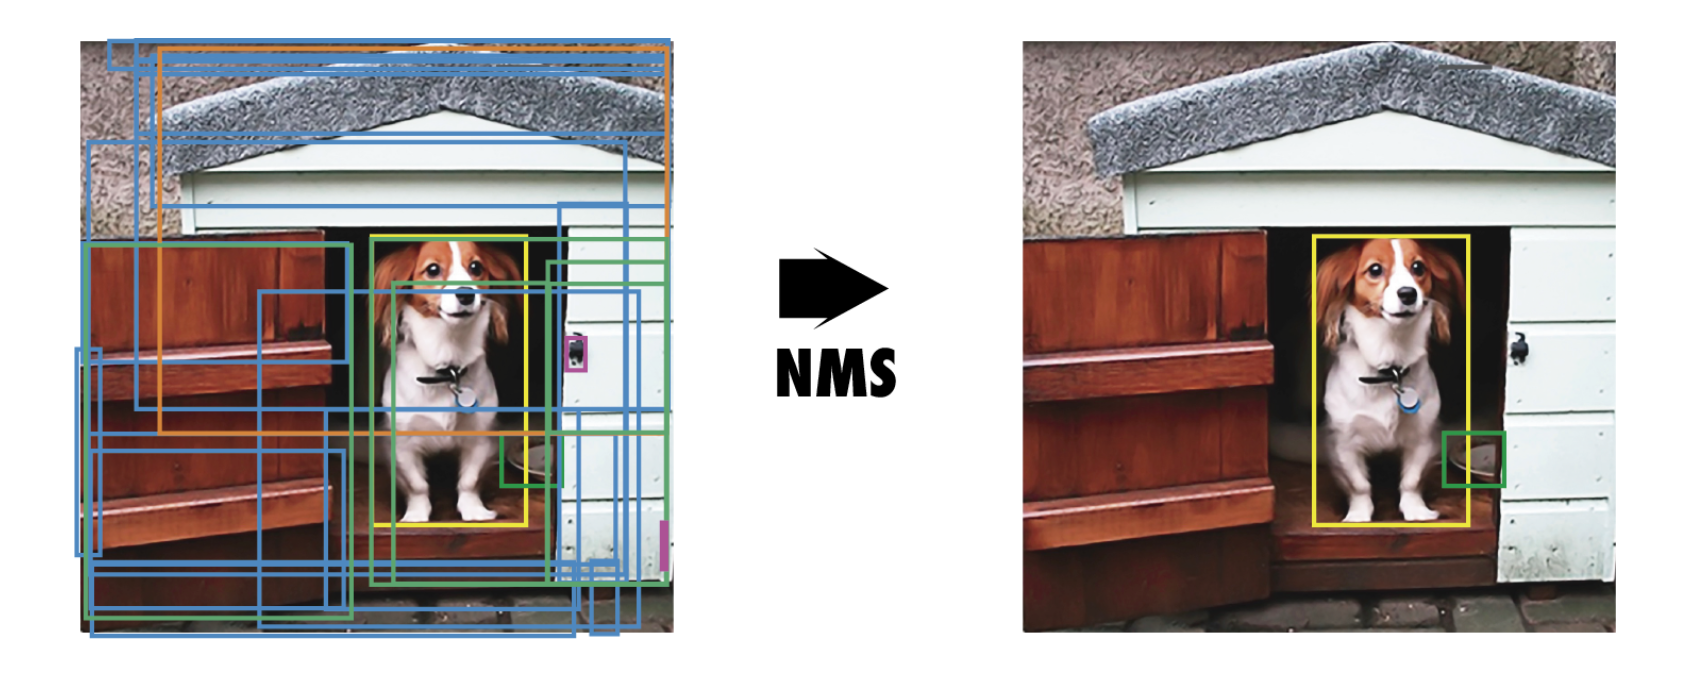
\includegraphics[scale=0.22]{Figures/NMS.png}
    \caption{Suppression des non-maximaux (NMS). a) Illustre la sortie typique d'un modèle de détection d'objets contenant plusieurs boîtes superposées. b) Illustre la sortie après l'application de la suppression des non-maximaux (NMS).}
    \label{fig:NMS}
\end{figure}
\vspace{0.6cm}

On va maintenant procéder à la description des différents modèles appartenant à la famille YOLO.

\section{YOLO: You Only Look Once}

L'article "YOLO" de Joseph Redmon et al., publié à CVPR 2016 \cite{38}, a présenté pour la première fois une approche en temps réel pour la détection d'objets de bout en bout. Le nom YOLO signifie "You Only Look Once", ce qui fait référence au fait qu'il était capable d'accomplir la tâche de détection en une seule passe du réseau, contrairement aux approches précédentes qui utilisaient soit des fenêtres glissantes suivies d'un classifieur nécessitant des centaines ou des milliers d'exécutions par image, soit des méthodes plus avancées qui divisaient la tâche en deux étapes, où la première étape détectait les régions possibles contenant des objets ou proposait des régions, et la deuxième étape exécutait un classifieur sur les propositions. De plus, YOLO utilisait une sortie plus simple basée uniquement sur la régression pour prédire les sorties de détection, contrairement à Fast R-CNN \cite{39} qui utilisait deux sorties distinctes, une pour la classification des probabilités et une pour la régression des coordonnées des boîtes.

\subsection{Principe de YOLOv1}

YOLOv1 fonctionne en unifiant les étapes de détection d'objets en détectant simultanément toutes les boîtes englobantes. Pour ce faire, YOLO divise l'image d'entrée en une grille $S\times S$ et prédit $B$ boîtes englobantes de la même classe, avec leur confiance pour $C$ classes différentes par élément de grille. Chaque prédiction de boîte englobante est composée de cinq valeurs : $Pc, bx, by, bh, bw$ où $Pc$ est le score de confiance de la boîte qui reflète à quel point le modèle est confiant que la boîte contient un objet et à quel point la boîte est précise. Les coordonnées $bx$ et $by$ sont les centres de la boîte par rapport à la cellule de grille, et $bh$ et $bw$ sont la hauteur et la largeur de la boîte par rapport à l'image complète. La sortie de YOLO est un tenseur de $S \times S \times (B\times 5 + C)$, éventuellement suivi de la suppression des non-maximaux (NMS) pour éliminer les détections en double.
\vspace{0.2cm}\\
Dans l'article original sur YOLO, les auteurs ont utilisé l'ensemble de données PASCAL VOC \cite{36} qui contient 20 classes ($C = 20$); une grille de $7\times 7$ ($S = 7$) et au plus 2 classes par élément de grille ($B = 2$), ce qui donne une prédiction de sortie de $7\times 7\times 30$.
\vspace{0.2cm}\\
La Figure \ref{fig:Output} montre un vecteur de sortie simplifié en considérant une grille de trois par trois, trois classes et une classe unique par grille pour huit valeurs. Dans ce cas simplifié, la sortie de YOLO serait de $3 \times 3 \times 8$.
\vspace{0.2cm}\\
YOLOv1 a atteint une précision moyenne (AP) de 63,4 sur l'ensemble de données PASCAL VOC2007.

\begin{figure}[htbp]
    \centering
    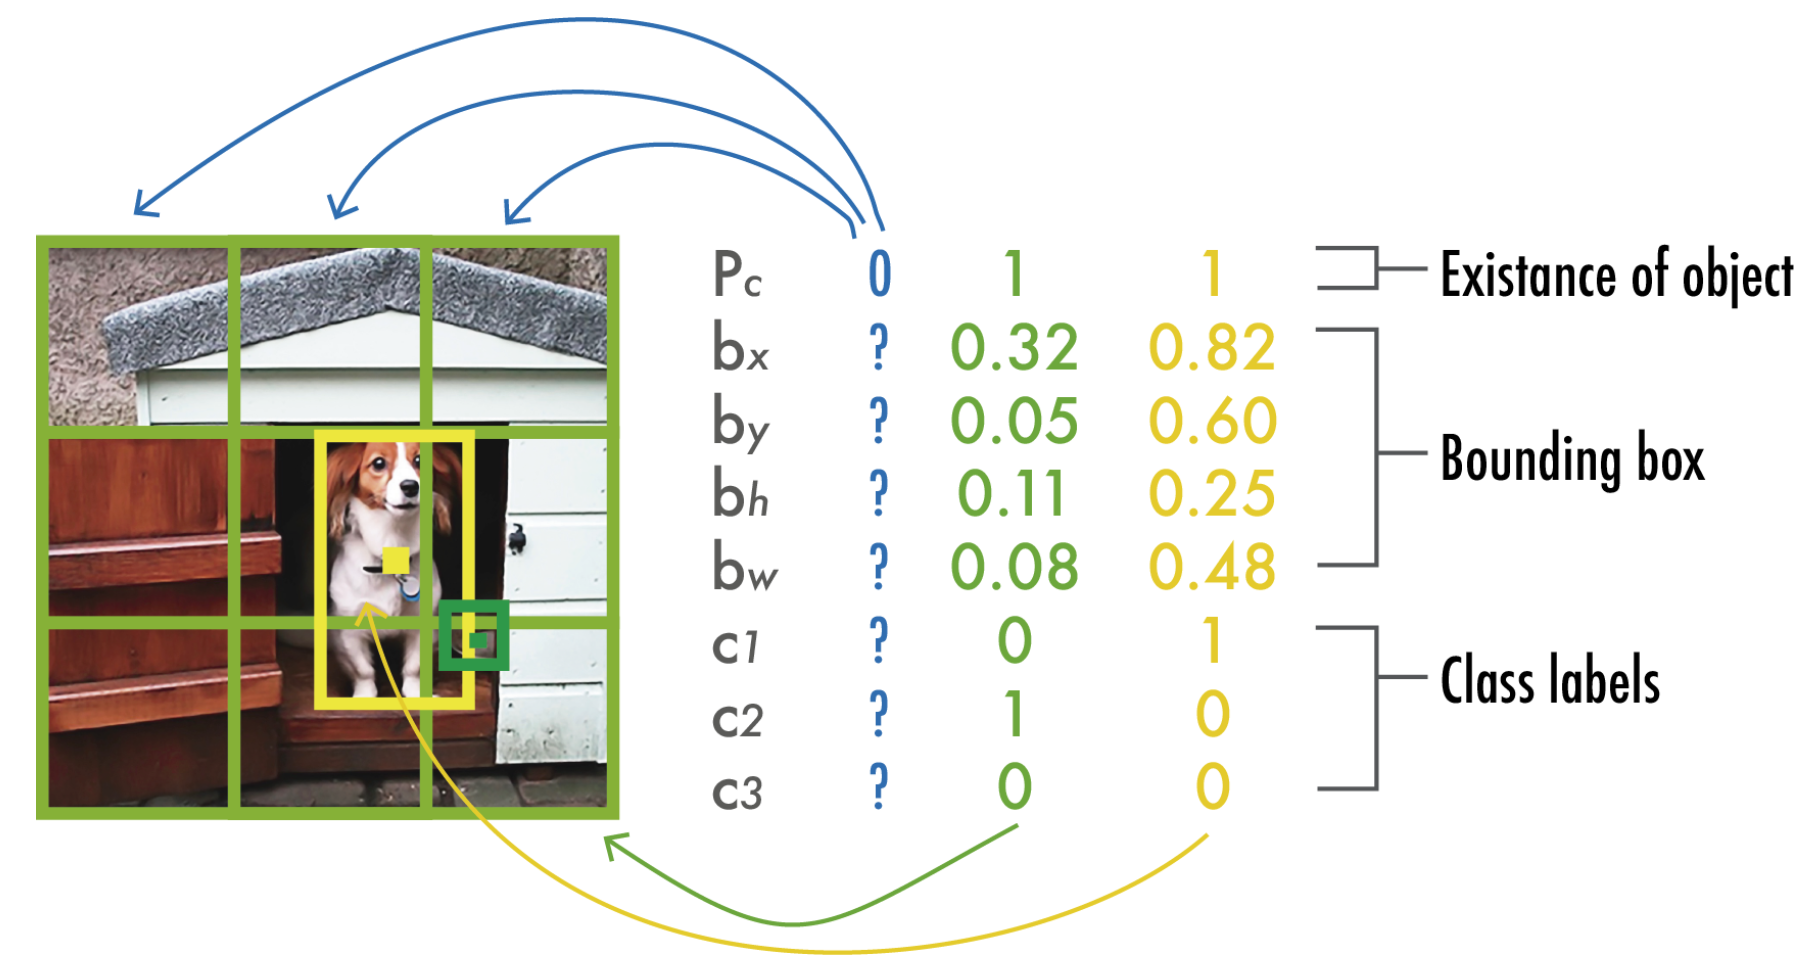
\includegraphics[scale=0.22]{Figures/Output.png}
    \caption{Prédiction de sortie de YOLO. La figure représente de manière simplifiée un modèle YOLO avec une grille de trois par trois, trois classes et une prédiction de classe unique par élément de grille, ce qui produit un vecteur de huit valeurs.}
    \label{fig:Output}
\end{figure}
\vspace{0.6cm}

\subsection{Architecture de YOLOv1}

L'architecture de YOLOv1 comprend 24 couches convolutionnelles suivies de deux couches entièrement connectées qui prédisent les coordonnées des boîtes englobantes et les probabilités. Toutes les couches utilisent des activations linéaires rectifiées avec fuite \cite{40}, à l'exception de la dernière qui utilise une fonction d'activation linéaire. Inspiré par GoogLeNet \cite{41} et Network in Network \cite{42}, YOLO utilise des couches de convolution $1\times 1$ pour réduire le nombre de cartes de caractéristiques et maintenir le nombre de paramètres relativement faible. Tableau \ref{tab:1} décrit l'architecture de YOLOv1 en tant que couches d'activation. Les auteurs ont également introduit un modèle plus léger appelé Fast YOLO, composé de neuf couches convolutionnelles.

\begin{table}[htbp]
\centering
\caption{Architecture de YOLO. Comprend 24 couches de convolution combinant des convolutions de $3 \times 3$ avec des convolutions de $1 \times 1$ pour la réduction des canaux. La sortie est une couche entièrement connectée qui génère une grille de $7 \times 7$ avec 30 valeurs pour chaque cellule de la grille afin de pouvoir accueillir dix coordonnées de boîtes englobantes (2 boîtes) avec 20 catégories.}
\begin{adjustbox}{width=0.65\textwidth}
$\begin{array}{@{}lllll@{}}
\hline & \text { Type } & \text { Filtre } & \text { Taille/Stride } & \text { Sortie } \\
\hline & \text { Conv } & 64 & 7 \times 7 / 2 & 224 \times 224 \\
& \text { Max Pool } & \text { } & 2 \times 2 / 2 & 112 \times 112 \\
 & \text { Conv } & 192 & 3 \times 3 / 1 & 112 \times 112 \\
 & \text { Max Pool } &   & 2 \times 2 / 2 & 56 \times 56 \\
\Xhline{1pt}
\multirow{2}{4em}{1 \times} & \text { Conv } & 128 & 1 \times 1 / 1 & 56 \times 56 \\
& \text { Conv } & 256 & 3 \times 3 / 1 & 56 \times 56 \\
&\text { Conv } & 256 & 1 \times 1 / 1 & 56 \times 56 \\
&\text { Conv } & 512 & 3 \times 3 / 1 & 56 \times 56 \\
&\text { Max Pool } & \text {  } & 2 \times 2 / 2 & 28 \times 28 \\
\Xhline{1pt}
\multirow{2}{4em}{4 \times} & \text{ Conv } & 256 & 1 \times 1 / 1 & 28 \times 28 \\
& \text{ Conv } & 512 & 3 \times 3 / 1 & 28 \times 28 \\
\Xhline{1pt}
& \text{ Conv } & 512 & 1 \times 1 / 1 & 28 \times 28 \\
& \text{ Conv } & 1024 & 3 \times 3 / 1 & 28 \times 28 \\
& \text{ Max Pool } & 2 \times 2 / 2 & 14 \times 14 \\
\Xhline{1pt}
\multirow{2}{4em}{2 \times} & \text{ Conv } & 512 & 1 \times 1 / 1 & 14 \times 14 \\
& \text{ Conv } & 1024 & 3 \times 3 / 1 & 14 \times 14 \\
\Xhline{1pt}
& \text{ Conv } & 1024 & 3 \times 3 / 1 & 14 \times 14 \\
& \text{ Conv } & 1024 & 3 \times 3 / 2 & 7 \times 7 \\
& \text{ Conv } & 1024 & 3 \times 3 / 1 & 7 \times 7 \\
& \text{ Conv } & 1024 & 3 \times 3 / 1 & 7 \times 7 \\
& \text{ FC } &  & 4096 & 4096 \\
& \text{ Dropout 0.5 } &  &  & 4096 \\
& \text{ FC } &  & 7 \times 7 \times 30 & 7 \times 7 \times 30 \\
\hline
\end{array}$
\end{adjustbox}
\label{tab:1}
\end{table}

\subsection{Entraînement de YOLOv1}

Les auteurs ont pré-entraîné les 20 premières couches de YOLO à une résolution de $224 \times 224$ en utilisant le jeu de données ImageNet \cite{43}. Ensuite, ils ont ajouté les quatre dernières couches avec des poids initialisés aléatoirement et ont affiné le modèle avec les jeux de données PASCAL VOC 2007 et VOC 2012 \cite{36} à une résolution de $448 \times 448$ pour augmenter les détails et améliorer la précision de la détection d'objets.
\vspace{0.2cm}\\
En ce qui concerne les augmentations, les auteurs ont utilisé des mises à l'échelle et des translations aléatoires d'au plus 20\% de la taille de l'image d'entrée, ainsi que des variations aléatoires d'exposition et de saturation avec un facteur maximal de 1,5 dans l'espace colorimétrique HSV.
\vspace{0.2cm}\\
YOLOv1 utilisait une fonction de perte composée de plusieurs sommes des carrés des erreurs, comme illustré dans la Figure \ref{fig:cost}. Dans la fonction de perte, $\lambda_{coord} = 5$ est un facteur d'échelle qui donne plus d'importance aux prédictions des boîtes englobantes, et $\lambda_{noobj} = 0.5$ est un facteur d'échelle qui diminue l'importance des boîtes ne contenant pas d'objets.
\vspace{0.2cm}\\
Les deux premiers termes de la perte représentent la perte de localisation; ils calculent l'erreur dans les prédictions des emplacements $(x, y)$ et des tailles $(w, h)$ des boîtes englobantes. Notez que ces erreurs ne sont calculées que dans les boîtes contenant des objets (représentées par le terme $\mathds{1}^{obj}_{ij}$), pénalisant uniquement si un objet est présent dans cette cellule de la grille. Les troisième et quatrième termes de la perte représentent la perte de confiance; le troisième terme mesure l'erreur de confiance lorsque l'objet est détecté dans la boîte ($\mathds{1}^{obj}_{ij}$) et le quatrième terme mesure l'erreur de confiance lorsque l'objet n'est pas détecté dans la boîte ($\mathds{1}^{noobj}_{ij}$). Étant donné que la plupart des boîtes sont vides, cette perte est pondérée par le terme $\lambda_{noobj}$. Le dernier composant de perte est la perte de classification qui mesure l'erreur quadratique des probabilités conditionnelles de classe pour chaque classe, uniquement si l'objet apparaît dans la cellule ($\mathds{1}^{obj}_i$).

\begin{figure}[htbp]
    \centering
    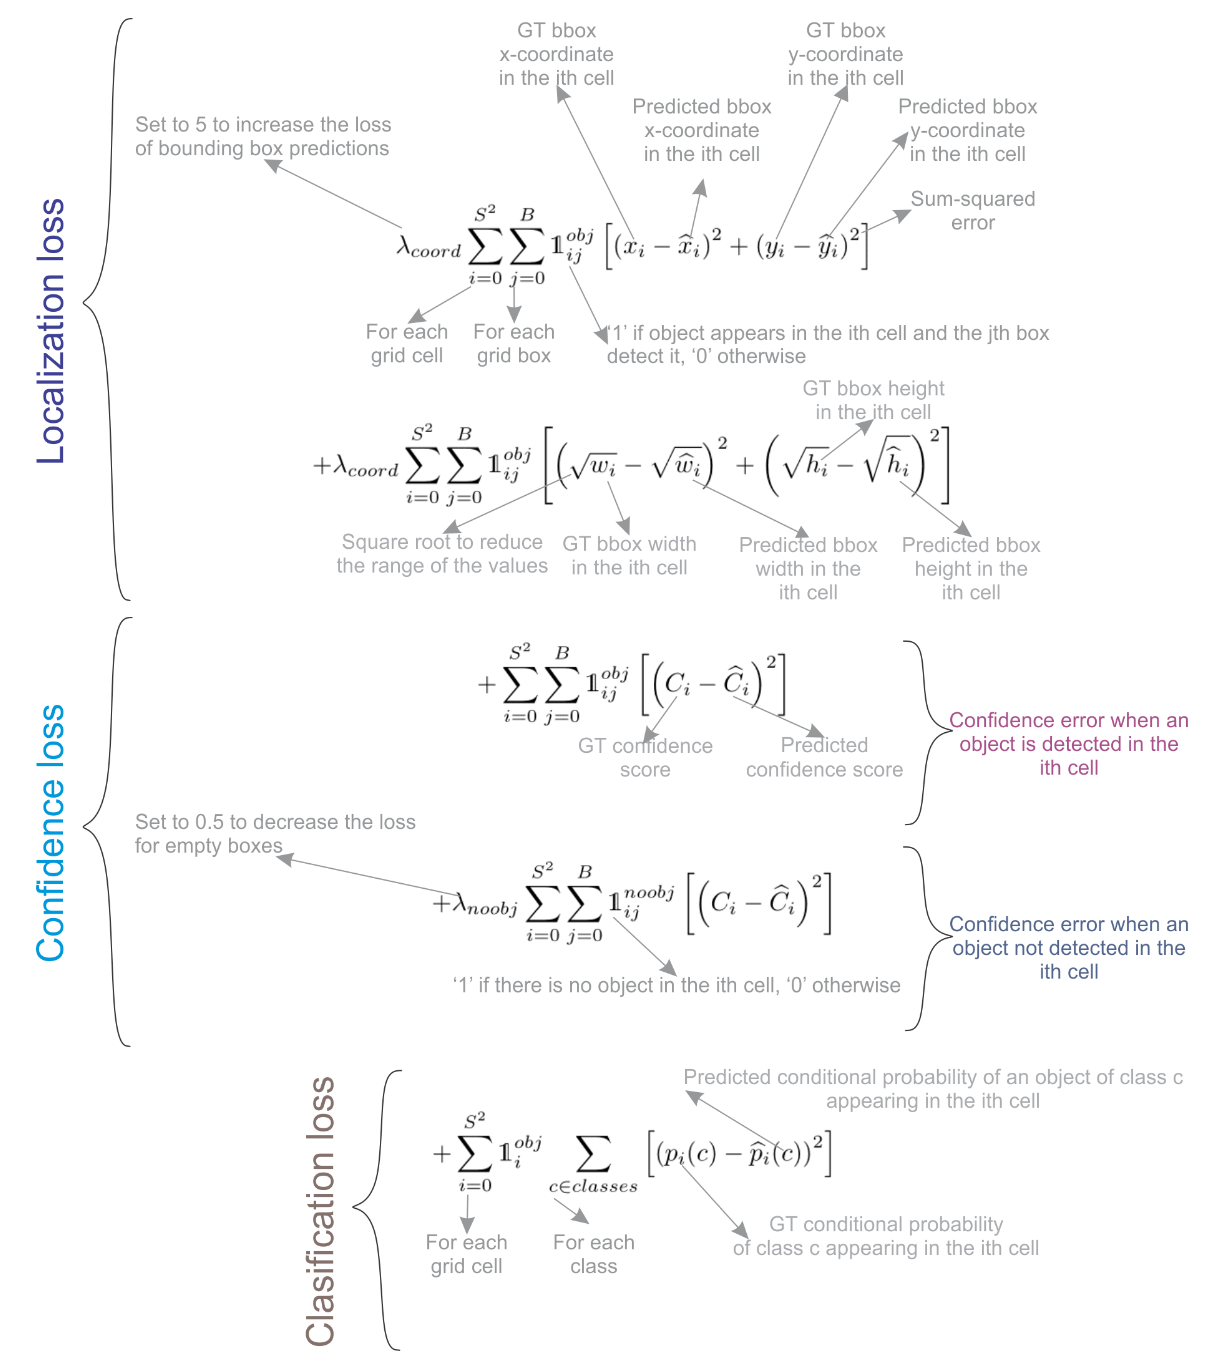
\includegraphics[scale=0.25]{Figures/cost.png}
    \caption{Fonction de coût YOLO. Comprend une perte de localisation pour les coordonnées des boîtes englobantes, une perte de confiance pour la présence ou l'absence d'objet, et une perte de classification pour l'exactitude de la prédiction de la catégorie.}
    \label{fig:cost}
\end{figure}
\vspace{0.6cm}

\subsection{YOLOv1 : Force \& Faiblesses}

La structure simple de YOLO, ainsi que sa méthode novatrice de régression en une seule étape sur l'image complète, lui ont permis d'être beaucoup plus rapide que les détecteurs d'objets existants, offrant ainsi des performances en temps réel.
\vspace{0.2cm}\\
Cependant, bien que YOLO soit plus rapide que tout autre détecteur d'objets, l'erreur de localisation était plus importante par rapport aux méthodes de pointe telles que Fast R-CNN \cite{39}. Trois principales causes expliquent cette limitation :
\begin{enumerate}
    \item Il ne pouvait détecter au maximum que deux objets de la même classe dans une cellule de la grille, limitant ainsi sa capacité à prédire des objets proches.
    \item Il avait du mal à prédire des objets avec des rapports d'aspect non observés dans les données d'entraînement.
    \item Il apprenait à partir de caractéristiques d'objets grossières en raison des couches de sous-échantillonnage.
\end{enumerate}


\section{YOLOv2 : Meilleur, plus Rapide \& plus Performant}

YOLOv2 a été publié à CVPR 2017 \cite{44} par Joseph Redmon et Ali Farhadi. Il présentait plusieurs améliorations par rapport au YOLO original, le rendant meilleur tout en conservant sa rapidité, et également plus performant - capable de détecter 9000 catégories! Les améliorations étaient les suivantes :\\
\begin{enumerate}
    \item \textbf{Normalisation par lots} (batch normalization) sur toutes les couches de convolution, améliorant la convergence et agissant comme un régulariseur pour réduire le surajustement (overfitting).
    \item \textbf{Classifieur à haute résolution}. À l'instar de YOLOv1, le modèle a été pré-entraîné avec ImageNet à une résolution de $224 \times 224$. Cependant, cette fois-ci, il a été affiné pendant dix époques sur ImageNet avec une résolution de $448 \times 448$, améliorant ainsi les performances du réseau sur des entrées de résolution plus élevée.
    \item \textbf{Entièrement convolutif}. Les couches denses ont été supprimées et une architecture entièrement convolutive a été utilisée.
    \item \textbf{Utilisation de boîtes d'ancrage pour prédire les boîtes englobantes}. Ils ont utilisé un ensemble de boîtes prédéfinies ou boîtes d'ancrage, qui sont des boîtes avec des formes prédéfinies utilisées pour correspondre aux formes prototypiques des objets, comme illustré dans la Figure \ref{fig:anchor}. Plusieurs boîtes d'ancrage sont définies pour chaque cellule de grille, et le système prédit les coordonnées et la classe pour chaque boîte d'ancrage. La taille de la sortie du réseau est proportionnelle au nombre de boîtes d'ancrage par cellule de grille.
    \item \textbf{Clusters de dimensions}. Le choix de bonnes boîtes d'ancrage aide le réseau à apprendre à prédire des boîtes englobantes plus précises. Les auteurs ont appliqué une classification $k$-moyennes ($k$-means) sur les boîtes englobantes d'entraînement pour trouver de bonnes boîtes d'ancrage. Ils ont sélectionné cinq boîtes d'ancrage offrant un bon compromis entre le rappel et la complexité du modèle.
    \item \textbf{Prédiction directe de la position}. Contrairement à d'autres méthodes qui prédisaient des décalages \cite{45}, YOLOv2 a suivi la même philosophie et a prédit les coordonnées de l'emplacement par rapport à la cellule de grille. Le réseau prédit cinq boîtes englobantes pour chaque cellule, chacune avec cinq valeurs $t_x, t_y, t_w, t_h et t_o$, où $t_o$ est équivalent à $Pc$ de YOLOv1, et les coordonnées finales des boîtes englobantes sont obtenues comme illustré dans la Figure \ref{fig:bounding}.
    \item \textbf{Caractéristiques plus fines}. YOLOv2, par rapport à YOLOv1, a supprimé une couche de pooling pour obtenir une carte de caractéristiques ou une grille de $13 \times 13$ pour des images d'entrée de $416 \times 416$. YOLOv2 utilise également une couche de passage qui prend la carte de caractéristiques de taille $26 \times 26 \times 512$ et la réorganise en empilant les caractéristiques adjacentes dans des canaux différents au lieu de les perdre via un sous-échantillonnage spatial. Cela génère des cartes de caractéristiques de taille $13 \times 13 \times 2048$ concaténées dans la dimension des canaux avec les cartes de taille inférieure $13 \times 13 \times 1024$ pour obtenir des cartes de caractéristiques de taille $13 \times 13 \times 3072$. Veuillez consulter le Tableau \ref{tab:2} pour les détails architecturaux.
    \item \textbf{Entraînement multi-échelle}. Étant donné que YOLOv2 n'utilise pas de couches entièrement connectées, les entrées peuvent avoir différentes tailles. Pour rendre YOLOv2 robuste à différentes tailles d'entrée, les auteurs ont entraîné le modèle de manière aléatoire en modifiant la taille de l'entrée - de $320 \times 320$ jusqu'à $608 \times 608$ - tous les dix lots.
\end{enumerate}

\vspace{0.2cm}\\

Avec toutes ces améliorations, YOLOv2 a obtenu une précision moyenne (AP) de 78,6\% sur le jeu de données PASCAL VOC2007, comparé à 63,4\% pour YOLOv1.

\begin{figure}[htbp]
    \centering
    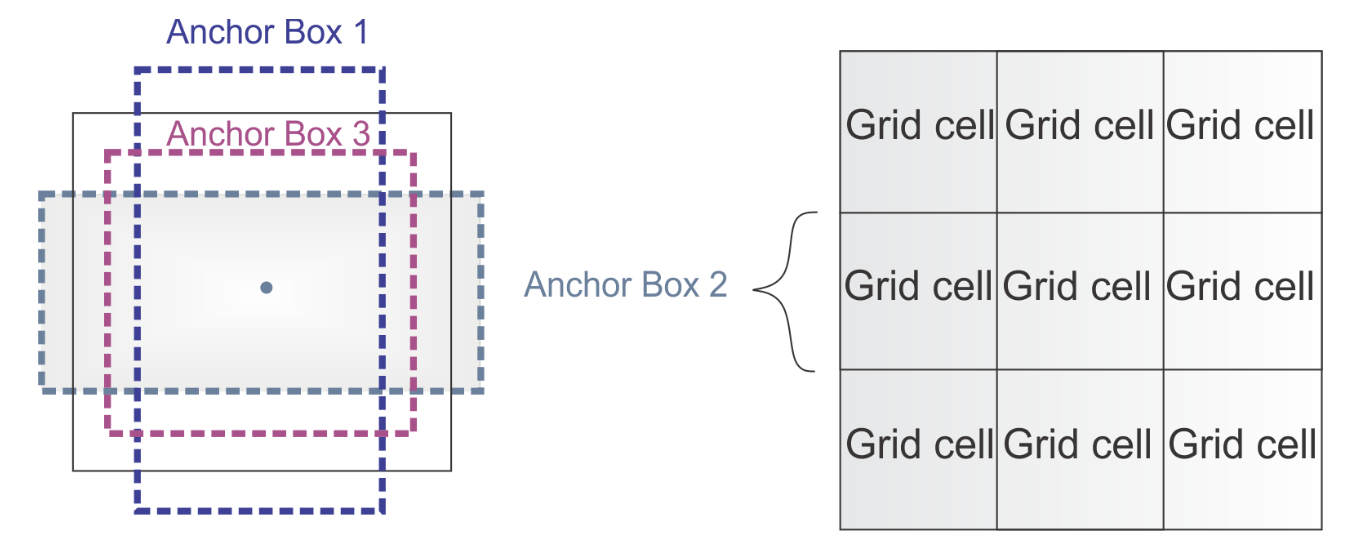
\includegraphics[scale=0.25]{Figures/anchor.png}
    \caption{Ancres. YOLOv2 définit plusieurs boîtes d'ancrage pour chaque cellule de la grille.}
    \label{fig:anchor}
\end{figure}


\begin{figure}[htbp]
    \centering
    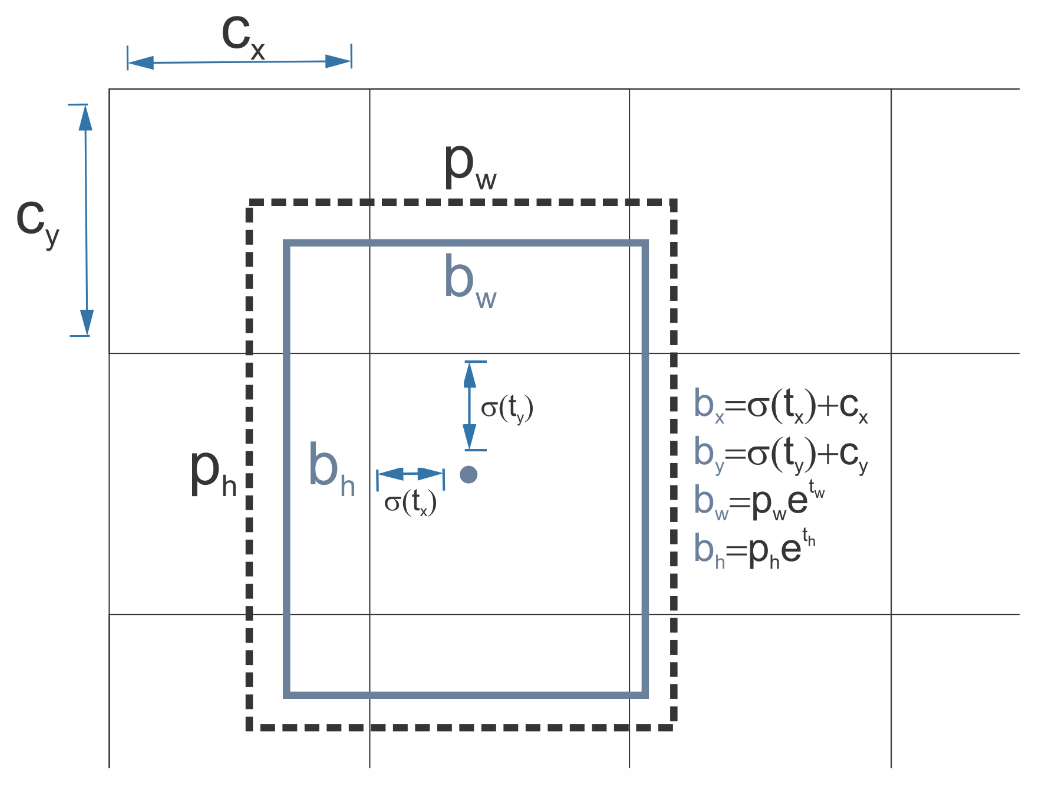
\includegraphics[scale=0.25]{Figures/bounding.png}
    \caption{Prédiction des boîtes englobantes. Les coordonnées du centre de la boîte sont obtenues à partir des valeurs prédites $t_x, t_y$ qui passent par une fonction sigmoïde et sont décalées par la position de la cellule de la grille $c_x, c_y$. La largeur et la hauteur de la boîte finale utilisent la largeur préalable $p_w$ et la hauteur préalable $p_h$, mises à l'échelle par $e^{t_w}$ et $e^{t_h}$ respectivement, où $t_w$ et $t_h$ sont prédits par YOLOv2.}
    \label{fig:bounding}
\end{figure}


\begin{table}[htbp]
\centering
\caption{Architecture de YOLOv2. La structure principale Darknet-19 (couches 1 à 23) est associée à la tête de détection composée des quatre dernières couches de convolution et de la couche de passage qui réorganise les caractéristiques de la $17^e$ sortie de $26 \times 26 \times 512$ en une sortie de $13 \times 13 \times 2048$, suivie d'une concaténation avec la $25^e$ couche. La dernière convolution génère une grille de $13 \times 13$ avec 125 canaux pour accueillir 25 prédictions (5 coordonnées $+$ 20 classes) pour cinq boîtes englobantes.}
\begin{adjustbox}{width=0.65\textwidth}
$\begin{array}{@{}lllll@{}}
\hline \text{ Nom } & \text { Type } & \text { Filtre } & \text { Taille/Stride } & \text { Sortie } \\
\hline
\ 1 & \text{Conv/BN} & 32 &  3 \times 3 / 1 & 416 \times 416 \times 32 \\
\ 2 & \text{Max Pool} & & 2 \times 2 / 2 & 208 \times 208 \times 32 \\
\ 3 & \text{Conv/BN} & 64 & 3 \times 3 / 1 & 208 \times 208 \times 64 \\
\ 4 & \text{Max Pool} & & 2 \times 2 / 2 & 104 \times 104 \times 64 \\
\ 5 & \text{Conv/BN} & 128 & 3 \times 3 / 1 & 104 \times 104 \times 128 \\
\ 6 & \text{Conv/BN} & 64 & 1 \times 1 / 1 & 104 \times 104 \times 64 \\
\ 7 & \text{Conv/BN} & 128 & 3 \times 3 / 1 & 104 \times 104 \times 128 \\
\ 8 & \text{Max Pool} & & 2 \times 2 / 2 & 52 \times 52 \times 128 \\
\ 9 & \text{Conv/BN} & 256 & 3 \times 3 / 1 & 52 \times 52 \times 256 \\
\ 10 & \text{Conv/BN} & 128 & 1 \times 1 / 1 & 52 \times 52 \times 128 \\
\ 11 & \text{Conv/BN} & 256 & 3 \times 3 / 1 & 52 \times 52 \times 256 \\
\ 12 & \text{Max Pool} & & 2 \times 2 / 2 & 26 \times 26 \times 256 \\
\ 13 & \text{Conv/BN} & 512 & 3 \times 3 / 1 & 26 \times 26 \times 512 \\
\ 14 & \text{Conv/BN} & 256 & 1 \times 1 / 1 & 26 \times 26 \times 256 \\
\ 15 & \text{Conv/BN} & 512 & 3 \times 3 / 1 & 26 \times 26 \times 512 \\
\ 16 & \text{Conv/BN} & 256 & 1 \times 1 / 1 & 26 \times 26 \times 256 \\
\ 17 & \text{Conv/BN} & 512 & 3 \times 3 / 1 & 26 \times 26 \times 512 \\
\ 18 & \text{Max Pool} & & 2 \times 2 / 2 & 13 \times 13 \times 512 \\
\ 19 & \text{Conv/BN} & 1024 & 3 \times 3 / 1 & 13 \times 13 \times 1024 \\
\ 20 & \text{Conv/BN} & 512 & 1 \times 1 / 1 & 13 \times 13 \times 512 \\
\ 21 & \text{Conv/BN} & 1024 & 3 \times 3 / 1 & 13 \times 13 \times 1024 \\
\ 22 & \text{Conv/BN} & 512 & 1 \times 1 / 1 & 13 \times 13 \times 512 \\
\ 23 & \text{Conv/BN} & 1024 & 3 \times 3 / 1 & 13 \times 13 \times 1024 \\
\hline
\ 24 & \text{Conv/BN} & 1024 & 3 \times 3 / 1 & 13 \times 13 \times 1024 \\
\ 25 & \text{Conv/BN} & 1024 & 3 \times 3 / 1 & 13 \times 13 \times 1024 \\
\ 26 & \text{Reorg layer 17} & & & 13 \times 13 \times 2048 \\
\ 27 & \text{Concat 25 and 26} & & & 13 \times 13 \times 3072 \\
\ 28 & \text{Conv/BN} & 1024 & 3 \times 3 / 1 & 13 \times 13 \times 1024 \\
\ 29 & \text{Conv} & 125 & 1 \times 1 / 1 & 13 \times 13 \times 125 \\
\hline
\end{array}$
\end{adjustbox}
\label{tab:2}
\end{table}


\subsection{Architecture de YOLOv2}


L'architecture de base utilisée par YOLOv2 est appelée Darknet-19, composée de 19 couches de convolution et de cinq couches de max-pooling. Tout comme l'architecture de YOLOv1, elle s'inspire du réseau Network in Network \cite{42}, utilisant des convolutions $1 \times 1$ entre les convolutions $3 \times 3$ pour réduire le nombre de paramètres. De plus, comme mentionné précédemment, ils utilisent la normalisation par lots (batch normalization) pour régulariser et faciliter la convergence. Le Tableau \ref{tab:2} présente l'ensemble de l'architecture Darknet-19 avec la tête de détection d'objets. YOLOv2 prédit cinq boîtes englobantes, chacune avec cinq valeurs et 20 classes lorsqu'il est utilisé avec l'ensemble de données PASCAL VOC.
\vspace{.2cm}\\
La tête de classification d'objets remplace les quatre dernières couches de convolution par une seule couche de convolution avec 1000 filtres, suivie d'une couche de pooling global moyen et d'une couche Softmax.

\subsection{YOLO9000 : Version Accrue de YOLOv2}

Les auteurs ont introduit une méthode pour l'entraînement de la classification et de la détection conjointes dans le même article. Ils ont utilisé les données d'étiquetage de détection provenant de COCO \cite{37} pour apprendre les coordonnées des boîtes englobantes et les données de classification provenant d'ImageNet afin d'augmenter le nombre de catégories qu'il peut détecter. Pendant l'entraînement, ils ont combiné les deux ensembles de données de telle sorte que lorsqu'une image d'entraînement de détection est utilisée, elle rétropropage le réseau de détection, et lorsqu'une image d'entraînement de classification est utilisée, elle rétropropage la partie de l'architecture liée à la classification. Le résultat est un modèle YOLO capable de détecter plus de 9000 catégories, d'où le nom YOLO9000.

\section{YOLOv3}
YOLOv3 \cite{46} a été publié dans ArXiv en 2018 par Joseph Redmon et Ali Farhadi. Il a introduit des modifications significatives ainsi qu'une architecture plus vaste afin de rivaliser avec les dernières avancées de l'état de l'art tout en maintenant des performances en temps réel. Dans la suite, nous décrivons les changements par rapport à YOLOv2.

\begin{enumerate}
    \item \textbf{Prédiction des boîtes englobantes} : Tout comme dans YOLOv2, le réseau prédit les quatre coordonnées ($t_x, t_y, t_w$ et $t_h$) pour chaque boîte englobante. Cependant, dans YOLOv3, une amélioration majeure est apportée en introduisant un score d'objectivité pour chaque boîte englobante, obtenu à l'aide d'une régression logistique. Ce score est établi à 1 pour l'anchor box présentant le chevauchement le plus élevé avec la boîte réelle, tandis que les autres boîtes d'ancrage se voient attribuer la valeur 0. Contrairement à Faster R-CNN \cite{45}, YOLOv3 associe uniquement une seule anchor box à chaque objet de la vérité terrain. De plus, en cas d'absence d'assignation d'une anchor box à un objet, cela n'entraîne qu'une perte de classification, sans perte de localisation ou de confiance.
    \item \textbf{Prédiction des classes} : Au lieu d'utiliser un softmax pour la classification, YOLOv3 utilise une perte d'entropie croisée (cross-entropy) binaire pour entraîner des classificateurs logistiques indépendants. Ainsi, le problème est formulé comme une classification multi-étiquettes. Cette modification permet d'attribuer plusieurs étiquettes à la même boîte, ce qui peut être nécessaire dans certains jeux de données complexes \cite{47} où des étiquettes se chevauchent. En guise d'exemple, un même objet peut être à la fois une personne et un homme.
    \item \textbf{Nouvelle architecture de base} : YOLOv3 dispose d'un extracteur de caractéristiques plus grand composé de 53 couches de convolution avec des connexions résiduelles. La section \ref{sect:1} du papier décrit l'architecture plus en détail.
    \item \textbf{Spatial Pyramid Pooling} (\textbf{SPP}) : Bien que cela ne soit pas mentionné dans le papier, les auteurs ont également ajouté à l'extracteur de caractéristiques un bloc SPP modifié \cite{48} . Ce bloc concatène plusieurs sorties de max pooling sans sous-échantillonnage (pas $= 1$), chacune avec différentes tailles de noyaux $k \times k$, où $k = 1, 5, 9, 13$, ce qui permet d'obtenir un champ récepteur plus large. Cette version est appelée YOLOv3-spp et a été la version la plus performante, améliorant l'{AP$_{50}$} de 2,7\%.
    \item \textbf{Prédictions multi-échelles} : Similairement aux Feature Pyramid Networks \cite{49}, YOLOv3 prédit trois boîtes à trois échelles différentes. La section \ref{sect:2} du papier décrit en détail le mécanisme de prédiction multi-échelles.
    \item \textbf{Antécédents des boîtes englobantes} : Comme dans YOLOv2, les auteurs utilisent également la méthode des $k$-moyennes pour déterminer les antécédents des boîtes d'ancrage. La différence est que dans YOLOv2, ils utilisaient un total de cinq boîtes par cellule, tandis que dans YOLOv3, ils utilisent trois boxes pour trois échelles différentes.
\end{enumerate}

\subsection{Architecture de YOLOv3}
\label{sect:1}

L'architecture de base présentée dans YOLOv3 est appelée Darknet-53. Elle a remplacé toutes les couches de max-pooling par des convolutions avec pas et a ajouté des connexions résiduelles. Au total, elle comprend 53 couches de convolution. La Figure \ref{fig:v3} illustre les détails de l'architecture.
\vspace{.2cm}\\
Le noyau Darknet-53 parvient à des précisions Top-1 et Top-5 comparables à celles du modèle ResNet-152, mais avec une vitesse presque deux fois supérieure.

\begin{figure}[htbp]
    \centering
    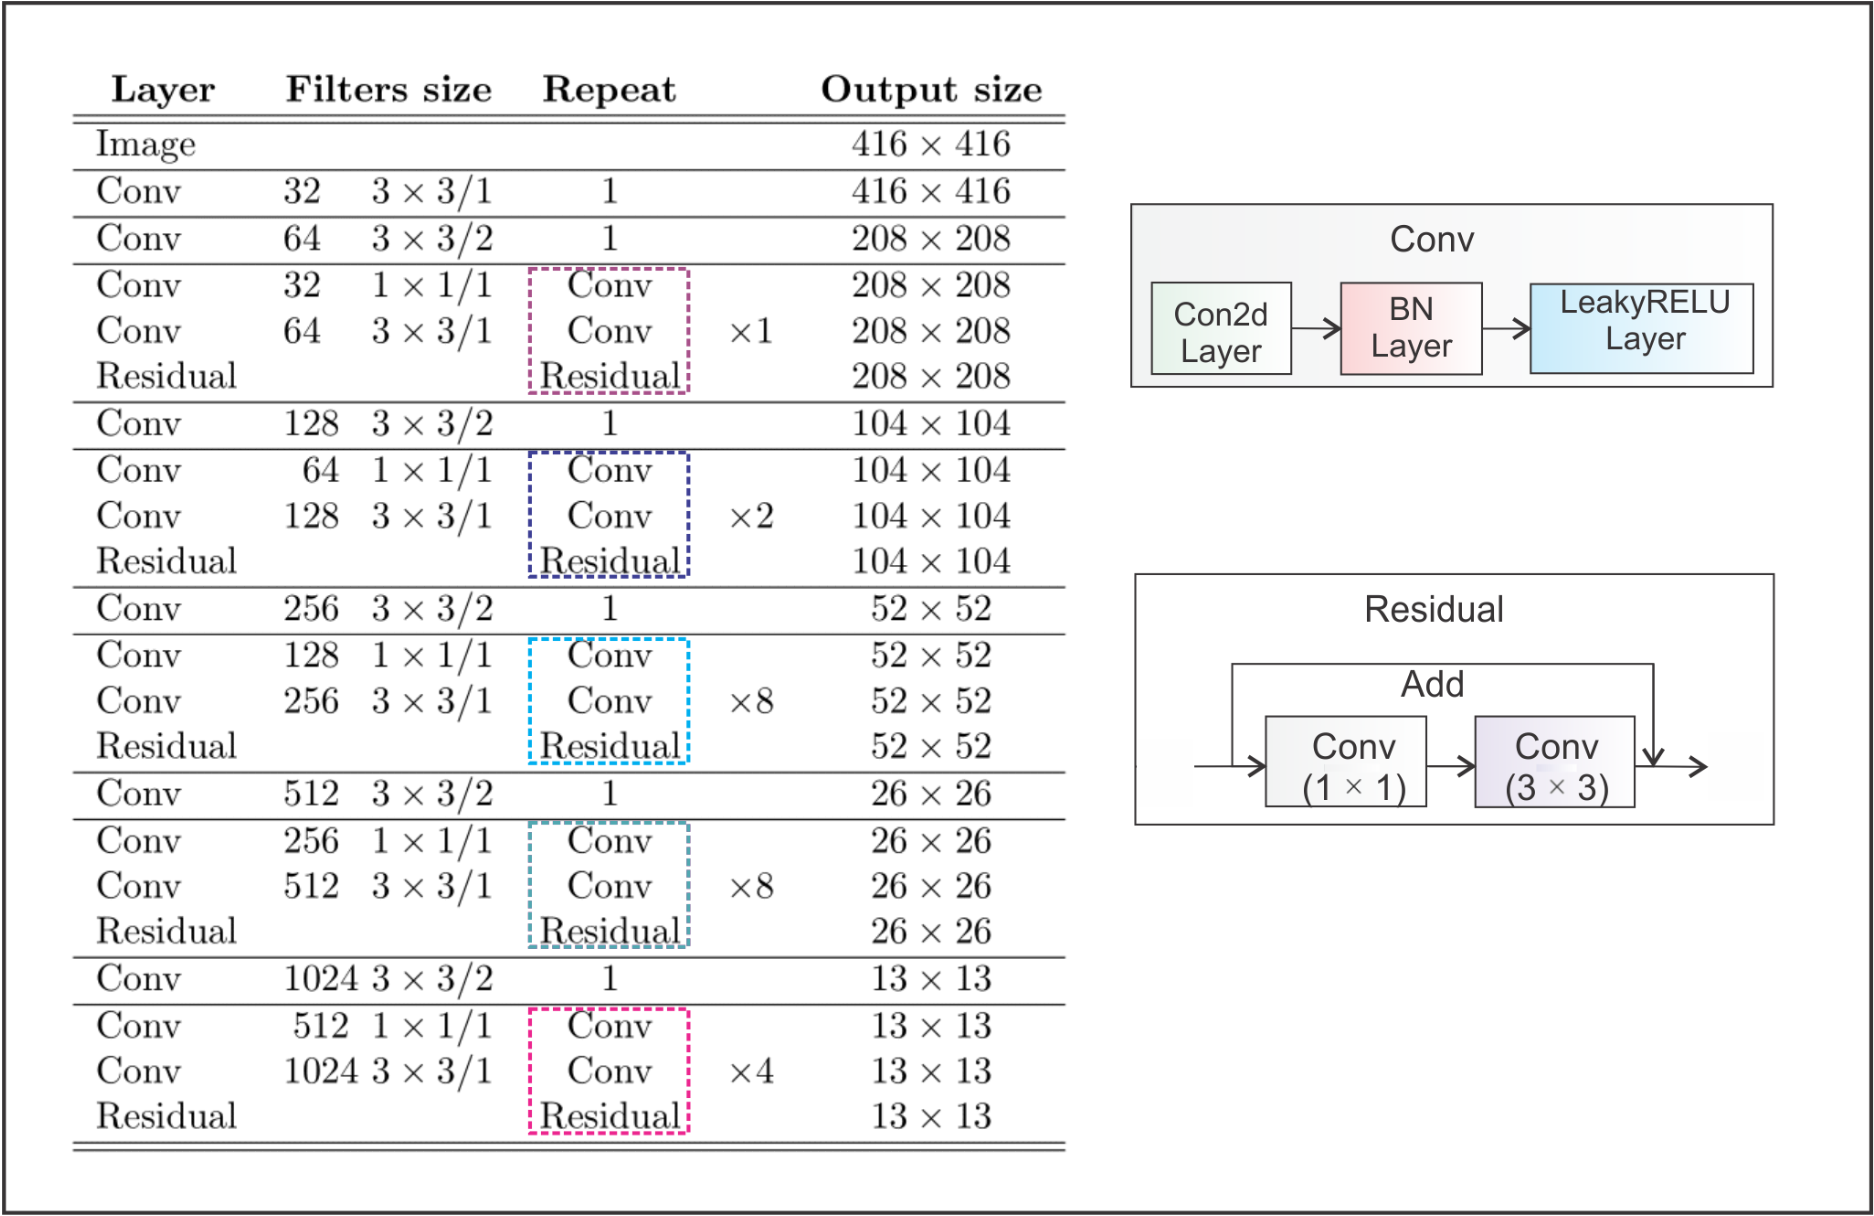
\includegraphics[scale=0.25]{Figures/v3.png}
    \caption{Noyau central de YOLOv3. Constitué de 53 couches de convolution, chacune étant dotée de la normalisation par lots (batch normalization) et de l'activation Leaky ReLU. De plus, des connexions résiduelles relient l'entrée des convolutions $1 \times 1$ dans l'ensemble du réseau à la sortie des convolutions $3 \times 3$. L'architecture présentée ici ne comprend que le noyau central, elle n'inclut pas la tête de détection composée de prédictions multi-échelles.}
    \label{fig:v3}
\end{figure}
\vspace{0.6cm}


\subsection{YOLOv3 : Prédictions Multi-Échelles}
\label{sect:2}

Outre une architecture plus grande, une caractéristique essentielle de YOLOv3 est la prédiction multi-échelle, c'est-à-dire des prédictions à plusieurs tailles de grille. Cela a permis d'obtenir des boîtes avec plus de détails et a considérablement amélioré la prédiction des petits objets, qui était l'une des principales faiblesses des versions précédentes de YOLO.
\vspace{.2cm}\\
L'architecture de détection multi-échelle illustrée dans la figure \ref{fig:multi} fonctionne comme suit : la première sortie marquée comme \textbf{y1} est équivalente à la sortie de YOLOv2, où une grille de $13 \times 13$ définit la sortie. La deuxième sortie \textbf{y2} est composée en concaténant la sortie après ($Res \times 4$) de Darknet-53 avec la sortie après ($Res \times 8$). Les cartes des caractéristiques ont des tailles différentes, c'est-à-dire $13 \times 13$ et $26 \times 26$, il y a donc une opération de sur-échantillonnage avant la concaténation. Enfin, en utilisant une opération de sur-échantillonnage, la troisième sortie \textbf{y3} concatène les cartes des caractéristiques de taille $26 \times 26$ avec les cartes des caractéristiques de taille $52 \times 52$.
\vspace{.2cm}\\
Pour le jeu de données COCO avec 80 catégories, chaque échelle fournit un tenseur de sortie avec une forme de $N \times N \times [3 \times (4 + 1 + 80)]$, où $N \times N$ est la taille de la carte des caractéristiques (ou de la cellule de grille), le 3 indique les boîtes par cellule et le $4 + 1$ inclut les quatre coordonnées et le score de présence de l'objet.

\begin{figure}[htbp]
    \centering
    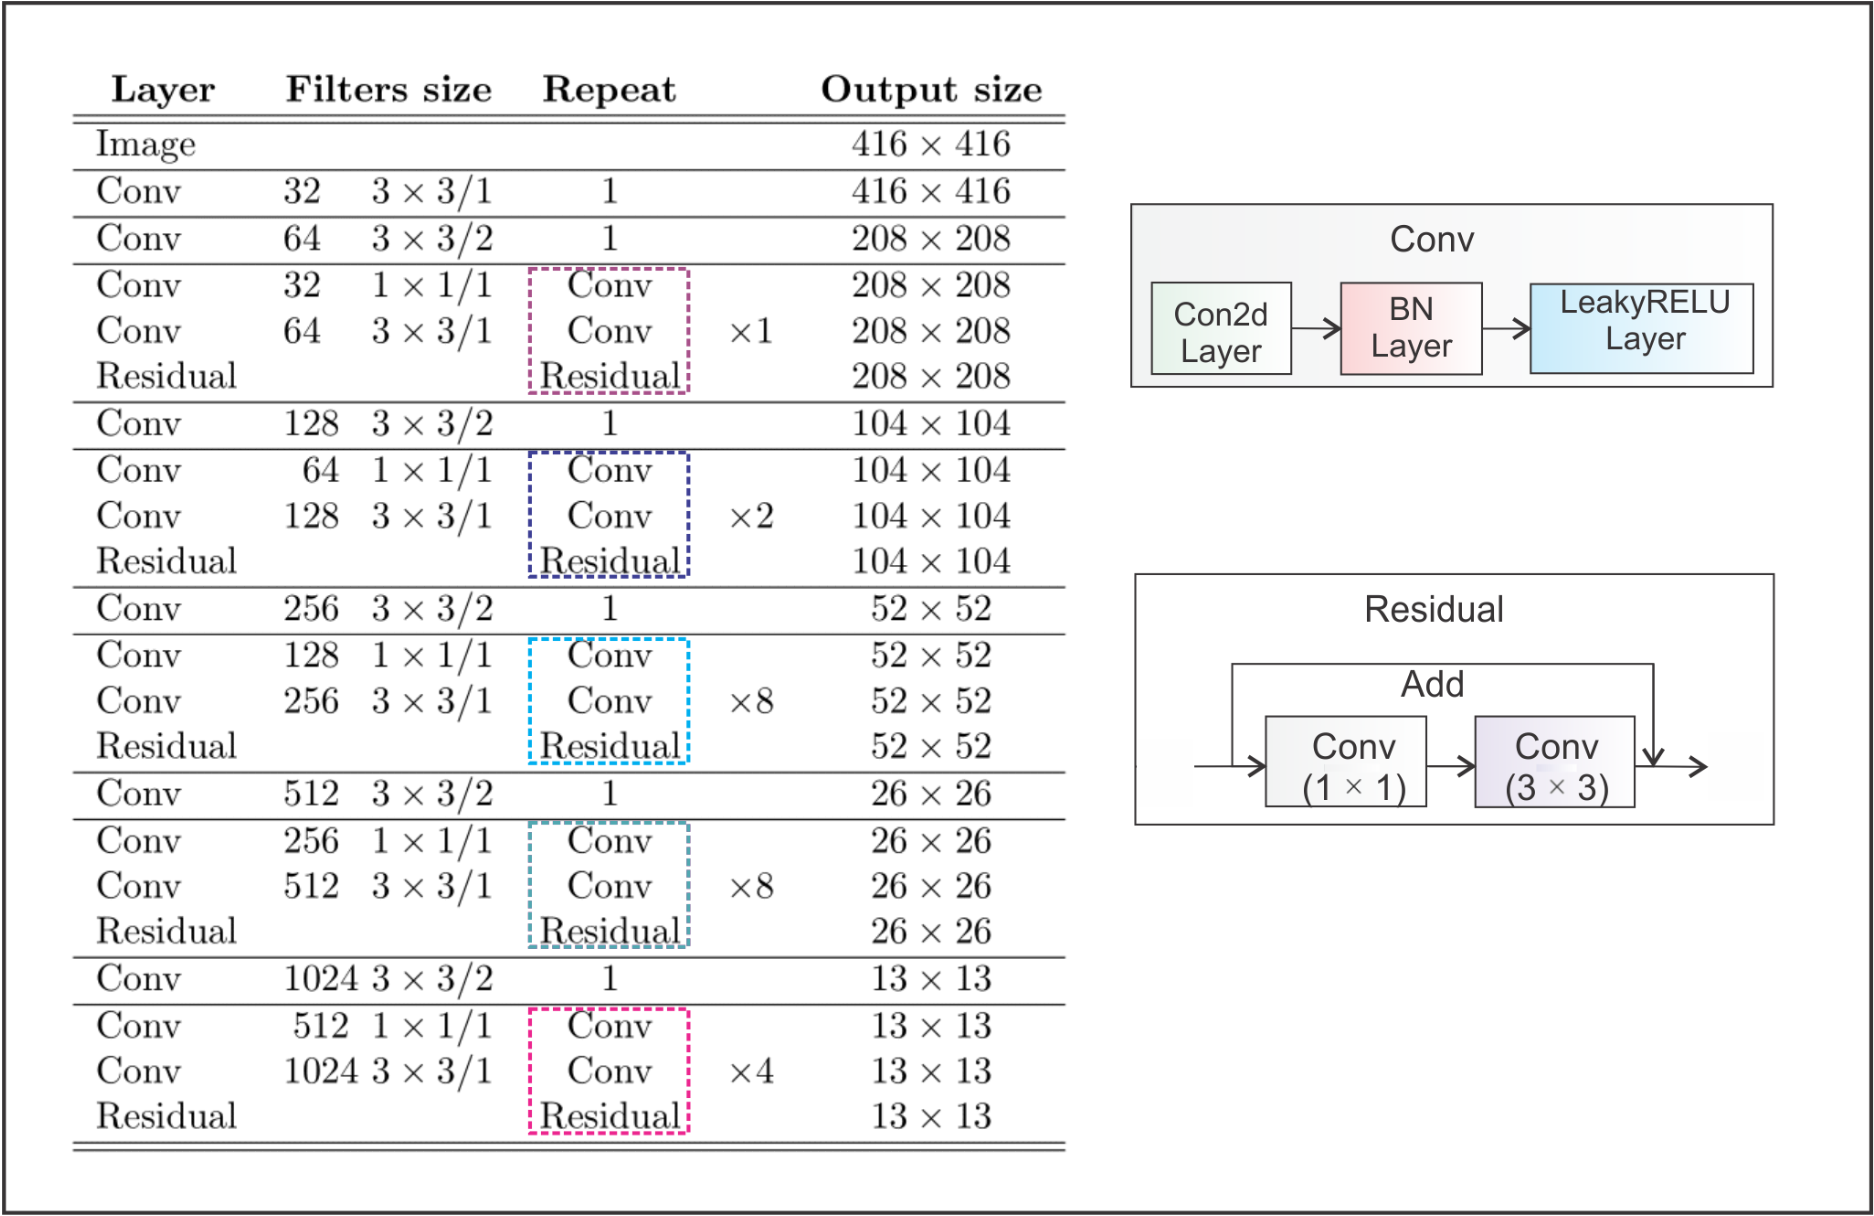
\includegraphics[scale=0.25]{Figures/v3.png}
    \caption{Architecture de détection multi-échelle de YOLOv3. La sortie de l'architecture Darknet-53 en est divisée en trois différentes marquées comme \textbf{y1}, \textbf{y2} et \textbf{y3}, chacune ayant une résolution augmentée. Les boîtes prédites finales sont filtrées à l'aide de la suppression non maximale. Les blocs CBL (Convolution-BatchNorm-Leaky ReLU) comprennent une couche de convolution avec normalisation par lots et activation Leaky ReLU. Les blocs Res comprennent un bloc CBL suivi de deux structures CBL avec une connexion résiduelle, comme illustré dans la figure \ref{fig:v3}.}
    \label{fig:multi}
\end{figure}


\subsection{Performance de YOLOv3}

Lorsque YOLOv3 a été publié, le référentiel pour la détection d'objets est passé de PASCAL VOC à Microsoft COCO \cite{37}. Par conséquent, à partir de ce moment-là, tous les modèles YOLO sont évalués sur l'ensemble de données MS COCO. YOLOv3-spp a obtenu une précision moyenne (AP) de 36,2\% et une précision moyenne à 50\% d'intersection sur union (AP$_{50}$) de 60,6\% à une vitesse de 20 images par seconde (FPS), ce qui le positionne à la pointe de la technologie de l'époque, tout en étant deux fois plus rapide.


\section{Architecture : Épine dorsale, Cou \& Tête}

À cette époque, l'architecture des détecteurs d'objets a commencé à être décrite en trois parties : l'épine dorsale, le cou et la tête. La figure \ref{fig:neck} présente un diagramme général de l'épine dorsale, du cou et de la tête.
\vspace{.2cm}\\
L'épine dorsale est responsable de l'extraction de caractéristiques utiles à partir de l'image d'entrée. Il s'agit généralement d'un réseau de neurones convolutionnel (CNN) entraîné sur une tâche de classification d'images à grande échelle, telle qu'ImageNet. L'épine dorsale capture des caractéristiques hiérarchiques à différentes échelles, avec des caractéristiques de bas niveau (par exemple, les contours et les textures) extraites dans les couches plus basses, et des caractéristiques de haut niveau (\textit{e.g.} les parties des objets et les informations sémantiques) extraites dans les couches plus profondes.
\vspace{.2cm}\\
Le cou est un composant intermédiaire qui relie l'épine dorsale à la tête. Il agrège et affine les caractéristiques extraites par l'épine dorsale, en se concentrant souvent sur l'amélioration de l'information spatiale et sémantique à différentes échelles. Le cou peut comprendre des couches de convolution supplémentaires, des réseaux de pyramides de caractéristiques (FPN) \cite{49} ou d'autres mécanismes visant à améliorer la représentation des caractéristiques.
\vspace{.2cm}\\
La tête est le composant final d'un détecteur d'objets ; elle est responsable de la génération de prédictions à partir des caractéristiques fournies par l'épine dorsale et le cou. Elle se compose généralement d'un ou plusieurs sous-réseaux spécifiques à la tâche qui effectuent la classification, la localisation et, plus récemment, la segmentation d'instance et l'estimation de pose. La tête traite les caractéristiques fournies par le cou, générant des prédictions pour chaque candidat d'objet. En fin de compte, une étape de post-traitement, telle que la suppression des non-maximaux (NMS), filtre les prédictions qui se chevauchent et ne conserve que les détections les plus confiantes.
\vspace{.2cm}\\
Dans le reste des modèles YOLO, on analyse les architectures en évoquant l'épine dorsale, le cou et la tête.

\begin{figure}[htbp]
    \centering
    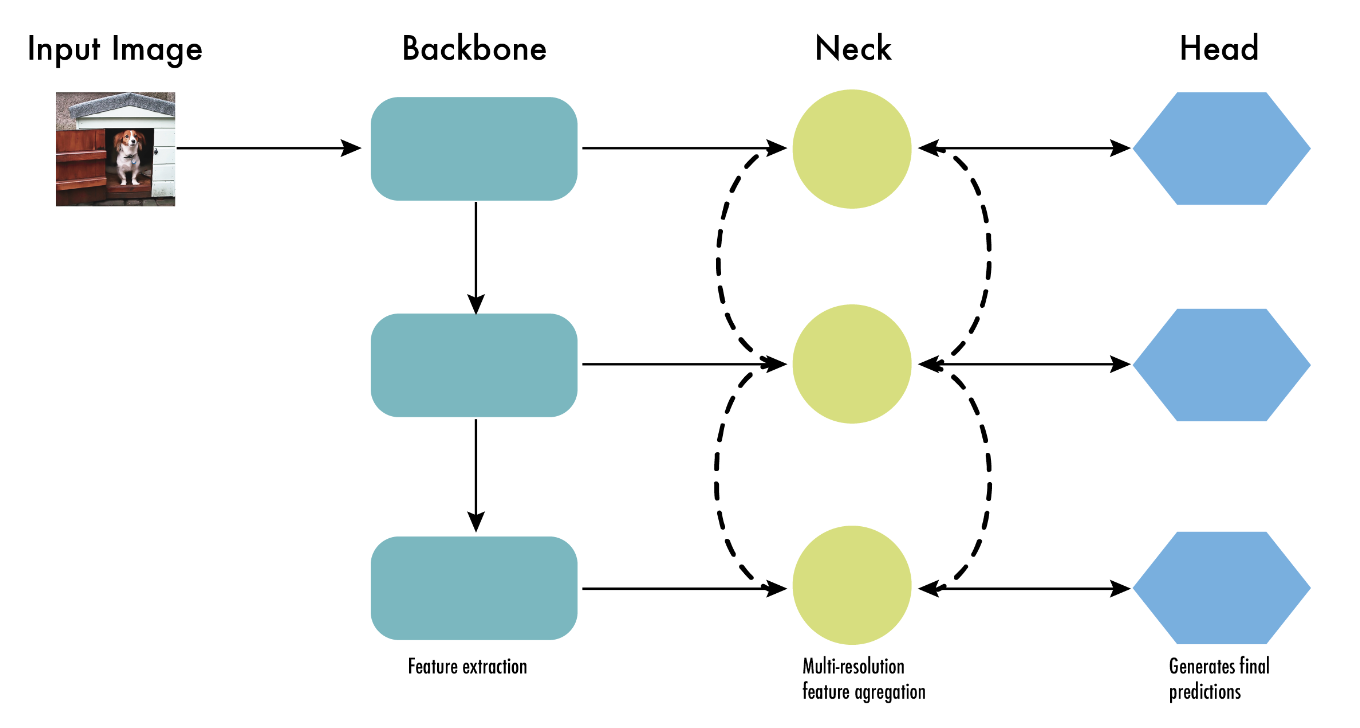
\includegraphics[scale=0.25]{Figures/neck.png}
    \caption{L'architecture des détecteurs d'objets modernes peut être décrite en termes d'épine dorsale, de cou et de tête.}
    \label{fig:neck}
\end{figure}
\vspace{0.6cm}

\section{YOLOv4}

Deux années se sont écoulées sans qu'une nouvelle version de YOLO ne soit publiée. Ce n'est qu'en avril 2020 qu'Alexey Bochkovskiy, Chien-Yao Wang et Hong-Yuan Mark Liao ont publié un article sur YOLOv4 dans ArXiv \cite{50}. Au début, il semblait étrange que de nouveaux auteurs présentent une nouvelle version "officielle" de YOLO ; cependant, YOLOv4 a conservé la même philosophie que YOLO, c'est-à-dire en temps réel, open source, à prise unique et utilisant le framework Darknet. Les améliorations apportées étaient si satisfaisantes que la communauté a rapidement adopté cette version en tant que YOLOv4 officiel.
\vspace{.2cm}\\
YOLOv4 a tenté de trouver un équilibre optimal en expérimentant de nombreux changements regroupés en deux catégories : les "bag-of-freebies" et les "bag-of-specials". Les "bag-of-freebies" sont des méthodes qui modifient uniquement la stratégie d'entraînement et augmentent le coût de l'entraînement, mais n'augmentent pas le temps d'inférence, le plus courant étant l'augmentation des données. En revanche, les "bag-of-specials" sont des méthodes qui augmentent légèrement le coût de l'inférence mais améliorent considérablement la précision. Parmi ces méthodes, on peut citer l'élargissement du champ récepteur \cite{48, 51,52}, la combinaison de caractéristiques \cite{53,49,54,55} et le post-traitement \cite{56,40,57,58}, entre autres.
\vspace{.2cm}\\
Nous résumons les principaux changements apportés à YOLOv4 dans les points suivants :
\begin{enumerate}
    \item \textbf{Architecture améliorée avec l'intégration de "bag-of-specials"} (\textbf{BoS}) : Les auteurs ont expérimenté plusieurs architectures pour le backbone, telles que ResNeXt50 \cite{59}, EfficientNet-B3 \cite{60} et Darknet-53. L'architecture qui a donné les meilleurs résultats était une modification de Darknet-53 avec des connexions partielles entre les différentes étapes (CSPNet) \cite{61} et une fonction d'activation Mish \cite{57} en tant que cou (Voir figure \ref{fig:v4}). Pour le cou, ils ont utilisé une version modifiée du spatial pyramid pooling (SPP) \cite{48} de YOLOv3-spp et des prédictions multi-échelles comme dans YOLOv3, mais avec une version modifiée du path aggregation network (PANet) \cite{62} et un module d'attention spatiale (SAM) \cite{63}. Pour la détection, ils ont utilisé des ancres comme dans YOLOv3. Par conséquent, le modèle a été appelé \textit{CSPDarknet53-PANet-SPP}. Les connexions partielles entre les différentes étapes (CSP) ajoutées à Darknet-53 permettent de réduire le calcul du modèle tout en maintenant la même précision. Le bloc SPP, comme dans YOLOv3-spp, augmente le champ récepteur sans affecter la vitesse d'inférence. La version modifiée de PANet concatène les caractéristiques au lieu de les additionner, comme dans l'article original sur PANet.
    \item \textbf{Intégration de "bag-of-freebies"} (\textbf{BoF}) \textbf{pour une approche d'entraînement avancée} : En plus des augmentations régulières telles que la luminosité aléatoire, le contraste, la mise à l'échelle, le recadrage, le retournement et la rotation, les auteurs ont mis en œuvre une augmentation par mosaïque qui combine quatre images en une seule, ce qui permet de détecter des objets en dehors de leur contexte habituel et réduit également la nécessité d'une grande taille de mini-lot pour la normalisation par lots. Pour la régularisation, ils ont utilisé DropBlock \cite{64} comme alternative à Dropout \cite{65} pour les réseaux de neurones convolutifs, ainsi que le lissage des étiquettes de classe \cite{66,67}. Pour le détecteur, ils ont ajouté la perte CIoU \cite{68} et la normalisation en mini-lot croisée (CmBN) pour collecter des statistiques sur l'ensemble du lot plutôt que sur des mini-lots individuels, comme dans la normalisation par lots classique \cite{69}.
    \item \textbf{Entraînement auto-contradictoire} (\textbf{SAT}) : Pour rendre le modèle plus robuste aux perturbations, une attaque adversaire est effectuée sur l'image d'entrée afin de créer une tromperie selon laquelle l'objet réel n'est pas présent dans l'image, tout en conservant l'étiquette d'origine pour détecter l'objet correct.
    \item \textbf{Optimisation des hyperparamètres avec des algorithmes génétiques} : Pour trouver les hyperparamètres optimaux utilisés pour l'entraînement, des algorithmes génétiques ont été utilisés sur les 10\% premières périodes, ainsi qu'un planificateur d'apprentissage à anneaux cosinus \cite{70} pour ajuster le taux d'apprentissage pendant l'entraînement. Celui-ci commence par une réduction lente du taux d'apprentissage, suivie d'une réduction plus rapide à mi-parcours, et se termine par une légère réduction.
\end{enumerate}
\vspace{.2cm}\\
Le Tableau \ref{tab:3} répertorie la sélection finale des BoFs et BoS pour le backbone et le détecteur.


\begin{figure}[htbp]
    \centering
    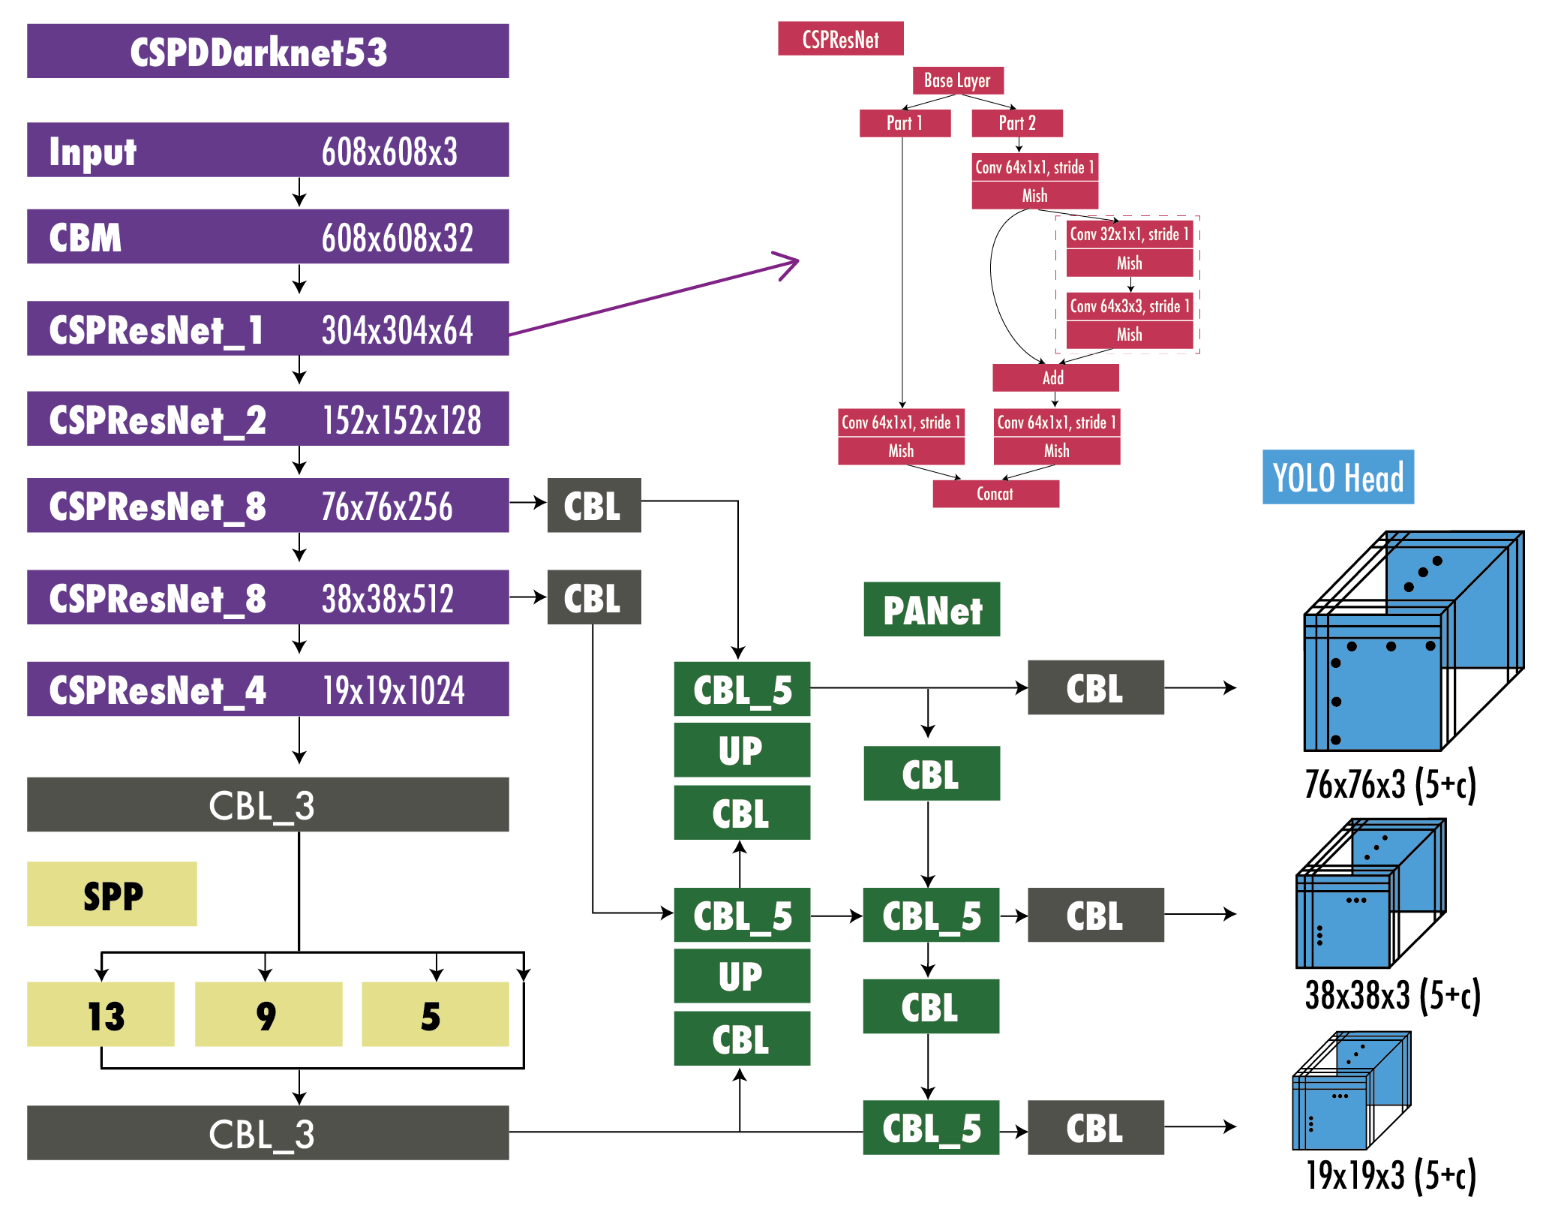
\includegraphics[scale=0.3]{Figures/v4.png}
    \caption{Architecture de YOLOv4 pour la détection d'objets. Les modules présents dans le diagramme sont les suivants : \textbf{CMB} (Convolution + Normalisation par lots + Activation Mish), \textbf{CBL} (Convolution + Normalisation par lots + Leaky ReLU), \textbf{UP} (upsampling), \textbf{SPP} (Spatial Pyramid Pooling) et \textbf{PANet} (Path Aggregation Network). Le diagramme est inspiré de \cite{71}.}
    \label{fig:v4}
\end{figure}
\vspace{0.6cm}


\begin{table}[htbp]
\centering
\caption{Sélection finale de bag-of-freebies (BoF) et de bag-of-specials (BoS) dans YOLOv4. Les BoFs sont des méthodes qui améliorent les performances sans coût d'inférence supplémentaire, mais qui nécessitent des temps d'entraînement plus longs. En revanche, les BoS sont des méthodes qui augmentent légèrement le coût d'inférence, mais qui améliorent considérablement la précision.}
\label{tab:3}
\begin{adjustbox}{width=0.9\textwidth}
$\begin{array}{@{}ll@{}}
\hline \textbf{ Backbone } & \textbf{ Détecteur } \\
\hline\\
\textbf{Bag-of-Freebies} & \textbf{Bag-of-Freebies} \\
\text{Augmentation des données} & \text{Augmentation des données} \\
\text{- Mosaic} & \text{- Mosaic} \\
\text{- CutMix} & \text{- Entraînement auto-adversaire} \\
\text{Regularisation} & \text{Perte CIoU} \\
\text{- DropBlock} & \text{Normalisation en mini-lots croisée (CmBN)} \\
\text{Lissage des étiquettes de classe} & \text{Élimination de la sensibilité à la grille} \\
& \text{Multiples ancres pour une vérité terrain unique} \\
& \text{Scheduler de réduction de cosinus} \\
& \text{Optimisation des hyperparamètres} \\
& \text{Formes d'entraînement aléatoires} \\
\\
\textbf{Bag-of-Specials} & \textbf{Bag-of-Specials} \\
\text{Activation Mish} & \text{Activation Mish} \\
\text{Connexions partielles entre les étapes (CSP)} & \text{Bloc de pyramide spatiale (SPP)} \\
\text{Connexions résiduelles pondérées multi-entrées} & \text{Module d'attention spatiale (SAM)} \\
& \text{Réseau d'agrégation de chemin (PAN)} \\
& \text{Distance-IoU \& Suppression non maximale} \\
\hline
\end{array}$
\end{adjustbox}
\end{table}

\subsection{Performance de YOLOv4}

Évalué sur le jeu de données MS COCO test-dev 2017, YOLOv4 a atteint un AP de 43,5\% et un AP$_{50}$ de 65,7\% à plus de 50 images par seconde sur une carte graphique NVIDIA V100.

\section{YOLOv5}

YOLOv5 \cite{72} a été publié quelques mois après YOLOv4 en 2020 par Glenn Jocher. Au moment de la rédaction de cet article, il n'y avait pas de publication scientifique sur YOLOv5, mais d'après le code, on sait qu'il utilise de nombreuses améliorations décrites dans la section YOLOv4, avec la principale différence étant qu'il a été développé en utilisant PyTorch plutôt que Darknet.
YOLOv5 est un logiciel open source maintenu activement par Ultralytics, avec plus de 250 contributeurs et de nouvelles améliorations régulières. YOLOv5 est facile à utiliser, à entraîner et à déployer. Ultralytics propose une version mobile pour iOS et Android ainsi que de nombreuses intégrations pour l'étiquetage, l'entraînement et le déploiement.
\vspace{.2cm}\\
YOLOv5 offre cinq versions d'échelle : YOLOv5n (nano), YOLOv5s (small), YOLOv5m (medium), YOLOv5l (large) et YOLOv5x (extra large).
\vspace{.2cm}\\
La version de YOLOv5 publiée au moment de la rédaction de cet article est la version 7.0, comprenant des versions de YOLOv5 capables de classification et de segmentation d'instance.

\subsection{Performance de YOLOv5}
Évalué sur le jeu de données MS COCO test-dev 2017, YOLOv5x a obtenu un AP de 50,7\% avec une taille d'image de 640 pixels. En utilisant une taille de lot (batch size) de 32, il peut atteindre une vitesse de 200 FPS sur une carte graphique NVIDIA V100. En utilisant une taille d'entrée plus grande de 1536 pixels, YOLOv5 atteint un AP de 55,8\%.

\section{Scaled-YOLOv4}
Un an après YOLOv4, les mêmes auteurs ont présenté Scaled-YOLOv4 \cite{73} lors de la conférence CVPR 2021. Contrairement à YOLOv4, Scaled YOLOv4 a été développé avec Pytorch au lieu de Darknet. La principale nouveauté était l'introduction de techniques de mise à l'échelle vers le haut et vers le bas. La mise à l'échelle vers le haut signifie produire un modèle qui augmente la précision au détriment de la vitesse ; en revanche, la mise à l'échelle vers le bas consiste à produire un modèle qui augmente la vitesse en sacrifiant la précision. De plus, les modèles réduits nécessitent moins de puissance de calcul et peuvent fonctionner sur des systèmes embarqués.
\vspace{.2cm}\\
L'architecture réduite a été appelée YOLOv4-tiny ; elle a été conçue pour les GPU d'entrée de gamme et peut fonctionner à 46 images par seconde sur un Jetson TX2 ou à 440 images par seconde sur un RTX2080Ti, atteignant un AP de 22\% sur MS COCO.
\vspace{.2cm}\\
L'architecture agrandie du modèle a été appelée YOLOv4-large, qui incluait trois tailles différentes : P5, P6 et P7. Cette architecture a été conçue pour les GPU en cloud et a atteint des performances de pointe, surpassant tous les modèles précédents \cite{74,75,76} avec un AP de 56\% sur MS COCO.


\section{YOLOR}
YOLOR \cite{77} a été publié sur ArXiv en mai 2021 par la même équipe de recherche que YOLOv4. YOLOR signifie \textit{You Only Learn One Representation}. Dans cet article, les auteurs ont adopté une approche différente ; ils ont développé une approche d'apprentissage multitâche qui vise à créer un modèle unique pour différentes tâches (\textit{e.g.} classification, détection, estimation de pose) en apprenant une représentation générale et en utilisant des sous-réseaux pour créer des représentations spécifiques à chaque tâche. Avec l'idée que la méthode d'apprentissage conjoint traditionnelle conduit souvent à une génération de caractéristiques sous-optimales, YOLOR vise à surmonter cela en encodant les connaissances implicites des réseaux neuronaux pour les appliquer à plusieurs tâches, de manière similaire à la façon dont les humains utilisent leurs expériences passées pour aborder de nouveaux problèmes. Les résultats ont montré que l'introduction de connaissances implicites dans le réseau neuronal bénéficie à toutes les tâches.
\vspace{.2cm}\\
Évalué sur le jeu de données MS COCO test-dev 2017, YOLOR a obtenu un AP de 55,4\% et un AP$_{50}$ de 73,3\% à 30 images par seconde sur une NVIDIA V100.

\section{YOLOX}

YOLOX \cite{78} a été publié sur ArXiv en juillet 2021 par une équipe de recherche de Megvii Technology. Développé en utilisant Pytorch et se basant sur YOLOV3 d'Ultralytics comme point de départ, il présente cinq changements principaux : une architecture sans ancrage, plusieurs positifs, une tête découplée, une attribution d'étiquettes avancée et des augmentations fortes. Il a atteint des résultats de pointe en 2021 avec un équilibre optimal entre vitesse et précision, avec un AP de 50,1\% à 68,9 images par seconde sur Tesla V100. Dans ce qui suit, on décrit les cinq principaux changements de YOLOX par rapport à YOLOv3 :


\begin{enumerate}
    \item \textbf{Sans ancrage}. Depuis YOLOv2, toutes les versions ultérieures de YOLO étaient des détecteurs basés sur des ancres. YOLOX, s'inspirant des détecteurs d'objets de pointe sans ancrage tels que CornerNet \cite{79}, CenterNet \cite{80} et FCOS \cite{81}, est revenu à une architecture sans ancrage, simplifiant ainsi le processus d'entraînement et de décodage. Le sans ancrage a augmenté l'AP de 0,9 points par rapport à la ligne de base YOLOv3.
    \item \textbf{Multiples positifs}. Pour compenser les grands déséquilibres produits par l'absence d'ancres, les auteurs utilisent un échantillonnage central \cite{81} où ils attribuent la zone centrale de $3 \times 3$ comme positifs. Cette approche a augmenté l'AP de 2,1 points.
    \item \textbf{Tête découplée}. Dans \cite{82,83}, il a été démontré qu'il pouvait y avoir un désalignement entre la confiance de classification et la précision de localisation. En raison de cela, YOLOX sépare ces deux éléments en deux têtes (comme illustré dans la figure \ref{fig:x}), l'une pour les tâches de classification et l'autre pour les tâches de régression, améliorant l'AP de 1,1 point et accélérant la convergence du modèle.
    \item \textbf{Attribution d'étiquettes avancée}. Dans \cite{84}, il a été démontré que l'attribution des étiquettes de vérité terrain pouvait être ambiguë lorsque les boîtes de plusieurs objets se chevauchent, et la procédure d'attribution a été formulée comme un problème de transport optimal (OT). YOLOX, s'inspirant de ce travail, a proposé une version simplifiée appelée simOTA. Ce changement a augmenté l'AP de 2,3 points.
    \item \textbf{Augmentations fortes}. YOLOX utilise les augmentations MixUP \cite{85} et Mosaic. Les auteurs ont constaté que la préparation préalable sur ImageNet n'était plus bénéfique après l'utilisation de ces augmentations. Les augmentations fortes ont augmenté l'AP de 2,4 points.
\end{enumerate}


\begin{figure}[htbp]
    \centering
    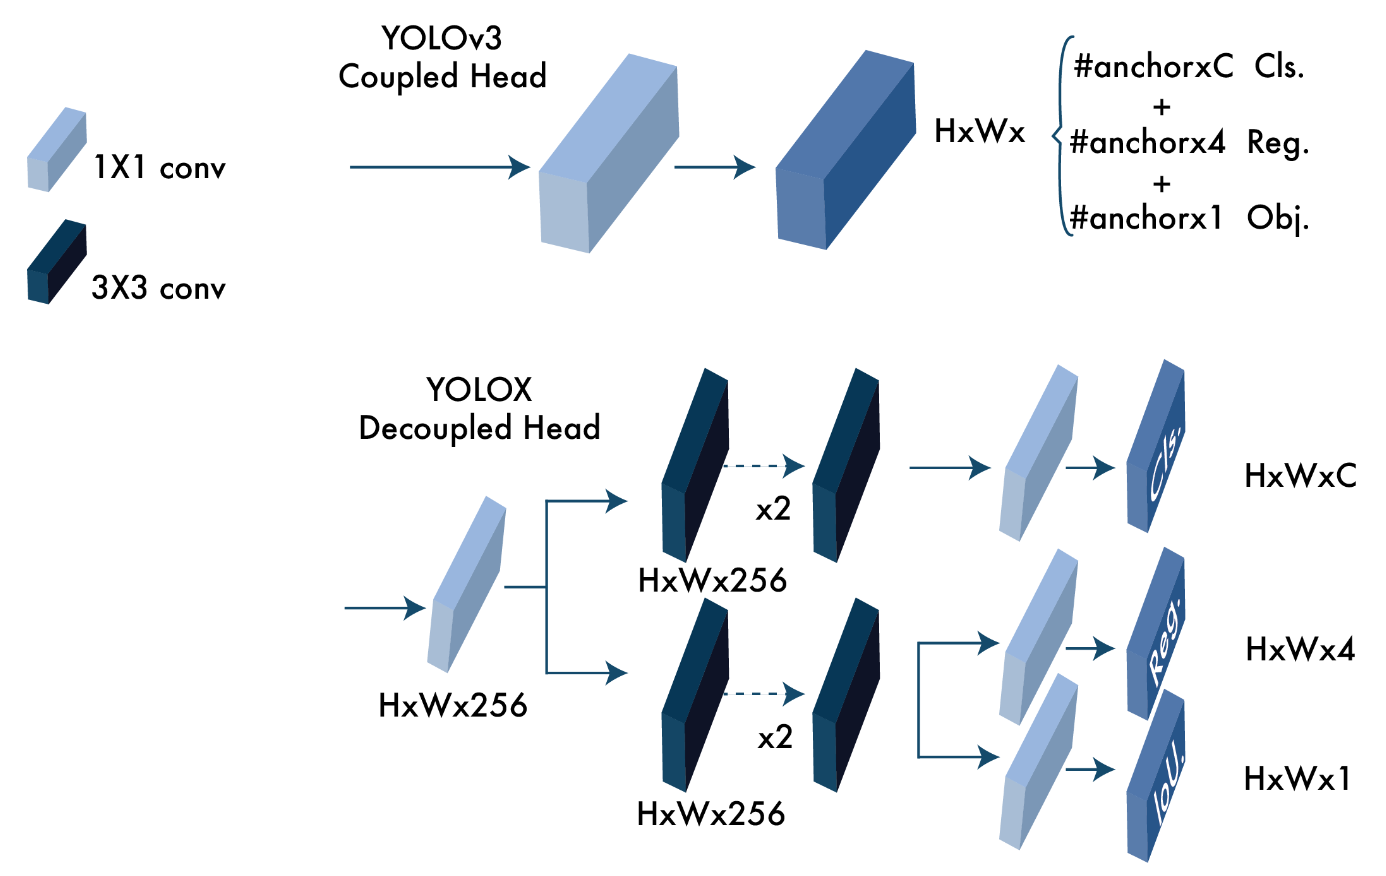
\includegraphics[scale=0.25]{Figures/X.png}
    \caption{Différence entre la tête de YOLOv3 et la tête découplée de YOLOX. Pour chaque niveau du FPN, ils ont utilisé une couche de convolution $1 \times 1$ pour réduire le nombre de canaux de caractéristiques à 256, puis ils ont ajouté deux branches parallèles avec deux couches de convolution $3 \times 3$ chacune pour les tâches de confiance de classement (classification) et de localisation (régression). La branche IoU est ajoutée à la tête de régression.}
    \label{fig:x}
\end{figure}
\vspace{0.6cm}

\section{YOLOv6}
YOLOv6 \cite{86} a été publié en septembre 2022 dans ArXiv par le département de l'IA de Meituan Vision. Tout comme YOLOv4 et YOLOv5, il propose différents modèles de différentes tailles pour des applications industrielles. Suivant la tendance des méthodes basées sur les points d'ancrage \cite{78,81}, YOLOv6 adopte un détecteur sans points d'ancrage. Les principales nouveautés de ce modèle sont résumées ci-dessous :

\begin{enumerate}
    \item \textbf{Nouvelle architecture de base basée sur RepVGG} \cite{87} appelée EfficientRep qui utilise une parallélisme plus élevé que les architectures précédentes de YOLO. Pour le neck, ils utilisent PAN \cite{62} amélioré avec des blocs RepBlocks \cite{87} ou CSPStackRep \cite{61} pour les modèles plus grands. Et inspirés par YOLOX, ils ont développé une tête découplée efficace.
    \item \textbf{Attribution des étiquettes} en utilisant l'approche d'apprentissage d'alignement de tâche introduite dans TOOD \cite{88}.
    \item \textbf{Nouvelles fonctions de perte pour la classification et la régression}. Ils utilisent une perte de classification VariFocal \cite{89} et une perte de régression SIoU \cite{90}/GIoU \cite{91}.
    \item \textbf{Stratégie d'auto-distillation} pour les tâches de régression et de classification.
    \item \textbf{Schéma de quantification} pour la détection utilisant RepOptimizer \cite{92} et la distillation par canal \cite{93} qui ont contribué à obtenir un détecteur plus rapide.
\end{enumerate}

\subsection{Résultats de YOLOv6}
Évalué sur le jeu de données MS COCO test-dev 2017, YOLOv6-L a obtenu un AP de 52,5\% et un AP50 de 70\% à environ 50 images par seconde sur une NVIDIA Tesla T4.

\section{YOLOv7}
YOLOv7 \cite{94} a été publié dans ArXiv en juillet 2022 par les mêmes auteurs que YOLOv4 et YOLOR. À l'époque, il surpassait tous les détecteurs d'objets connus en termes de vitesse et de précision dans une plage de 5 FPS à 160 FPS. Comme YOLOv4, il a été entraîné uniquement avec l'ensemble de données MS COCO, sans pré-entraînement des modèles de base. YOLOv7 a proposé plusieurs modifications d'architecture et une série de "bag-of-freebies", qui ont augmenté la précision sans affecter la vitesse d'inférence, seulement le temps d'entraînement.
\vspace{.2cm}\\
Les modifications d'architecture de YOLOv7 sont les suivantes :

\begin{itemize}
    \item[$\bullet$] \textbf{Extended efficient layer aggregation network (E-ELAN)}. ELAN \cite{95} est une stratégie qui permet à un modèle profond d'apprendre et de converger de manière plus efficace en contrôlant le chemin du gradient le plus court le plus long. YOLOv7 a proposé E-ELAN qui fonctionne pour les modèles avec des blocs de calcul empilés de manière illimitée. E-ELAN combine les caractéristiques de différents groupes en les mélangeant et en fusionnant leur cardinalité pour renforcer l'apprentissage du réseau sans détruire le chemin de gradient original.
    \item[$\bullet$] \textbf{Mise à l'échelle du modèle pour les modèles basés sur la concaténation}. La mise à l'échelle génère des modèles de différentes tailles en ajustant certaines caractéristiques du modèle. L'architecture de YOLOv7 est une architecture basée sur la concaténation dans laquelle les techniques de mise à l'échelle standard, telles que la mise à l'échelle de la profondeur, provoquent un changement de ratio entre le canal d'entrée et le canal de sortie d'une couche de transition, ce qui entraîne une diminution de l'utilisation matérielle du modèle. YOLOv7 a proposé une nouvelle stratégie de mise à l'échelle des modèles basés sur la concaténation, dans laquelle la profondeur et la largeur du bloc sont mises à l'échelle avec le même facteur pour maintenir la structure optimale du modèle.
\end{itemize}

Les "bag-of-freebies" utilisés dans YOLOv7 comprennent :

\begin{itemize}
    \item[$\bullet$] \textbf{Convolution re-paramétrisée planifiée}. Comme dans YOLOv6, l'architecture de YOLOv7 s'inspire également des convolutions re-paramétrisées (RepConv) \cite{87}. Cependant, ils ont constaté que la connexion identité dans RepConv détruit la résiduelle dans ResNet \cite{53} et la concaténation dans DenseNet \cite{96}. Pour cette raison, ils ont supprimé la connexion identité et l'ont appelée RepConvN.
    \item[$\bullet$] \textbf{Attribution d'étiquettes grossières pour la tête auxiliaire et attribution d'étiquettes fines pour la tête principale}. La tête principale est responsable de la sortie finale, tandis que la tête auxiliaire aide à l'entraînement.
    \item[$\bullet$] \textbf{Normalisation par lots (batch normalization) dans la couche conv-bn-activation}. Cela intègre la moyenne et la variance de la normalisation par lots dans le biais et le poids de la couche de convolution lors de l'inférence.
    \item[$\bullet$] \textbf{Connaissance implicite} inspirée de YOLOR \cite{77}.
    \item[$\bullet$] \textbf{Moyenne mobile exponentielle} comme modèle d'inférence final.
\end{itemize}


\subsection{Comparison avec YOLOv4 et YOLOR}
Dans cette section, on met en évidence les améliorations apportées par YOLOv7 par rapport aux modèles YOLO précédents développés par les mêmes auteurs.
\vspace{.2cm}\\
Par rapport à YOLOv4, YOLOv7 a réussi à réduire de 75\% le nombre de paramètres et de 36\% le calcul, tout en améliorant simultanément la précision moyenne (AP) de 1,5\%.
\vspace{.2cm}\\
En revanche, par rapport à YOLOv4-tiny, YOLOv7-tiny a réussi à réduire les paramètres et le calcul de 39\% et 49\% respectivement, tout en maintenant la même AP.
\vspace{.2cm}\\
Enfin, par rapport à YOLOR, YOLOv7 a réduit le nombre de paramètres et le calcul de 43\% et 15\% respectivement, tout en enregistrant une légère augmentation de 0,4\% de l'AP.

\subsection{Résultats de YOLOv7}
Évalué sur l'ensemble de données MS COCO test-dev 2017, YOLOv7-E6 a obtenu une précision moyenne (AP) de 55,9\% et un AP$_{50}$ de 73,5\% avec une taille d'entrée de 1280 pixels, à une vitesse de 50 images par seconde (FPS) sur un NVIDIA V100.


\section{DAMO-YOLO}
DAMO-YOLO \cite{97} a été publié en novembre 2022 par le groupe Alibaba. Inspiré par les technologies actuelles, DAMO-YOLO comprenait les éléments suivants :

\begin{itemize}
    \item[$\bullet$] \textbf{Recherche d'architecture neuronale} (\textbf{NAS}). Ils ont utilisé une méthode appelée MAE-NAS \cite{98} développée par Alibaba pour trouver automatiquement une architecture efficace.
    \item[$\bullet$] "\textbf{Neck}" (\textbf{cou}) \textbf{large}. Inspiré par GiraffeDet \cite{99}, CSPNet \cite{61} et ELAN \cite{95}, les auteurs ont conçu un neck qui peut fonctionner en temps réel appelé Efficient-RepGFPN.
    \item[$\bullet$] "\textbf{Head}" (\textbf{tête}) \textbf{petite}. Les auteurs ont constaté qu'un neck large et une tête petite donnent de meilleures performances, et ils n'ont laissé qu'une couche linéaire pour la classification et une pour la régression. Ils ont appelé cette approche ZeroHead.
    \item[$\bullet$] \textbf{Assignation des étiquettes AlignedOTA}. Les méthodes d'assignation dynamique des étiquettes, telles que OTA\cite{84} et TOOD\cite{88}, sont devenues populaires en raison de leurs améliorations significatives par rapport aux méthodes statiques. Cependant, le désalignement entre la classification et la régression reste un problème, en partie en raison du déséquilibre entre les pertes de classification et de régression. Pour résoudre ce problème, leur méthode AlignOTA introduit la focal loss \cite{75} dans le coût de classification et utilise l'IoU de la prédiction et de la boîte ground truth comme étiquette souple, permettant la sélection d'échantillons alignés pour chaque cible et résolvant le problème d'une perspective globale.
    \item[$\bullet$] \textbf{Distillation des connaissances}. Leur stratégie proposée se compose de deux étapes : le professeur guide l'élève dans la première étape et l'élève se perfectionne de manière indépendante dans la deuxième étape. De plus, ils intègrent deux améliorations dans l'approche de distillation : le module Align, qui adapte les caractéristiques de l'élève à la même résolution que celles du professeur, et la température dynamique par canal, qui normalise les caractéristiques du professeur et de l'élève pour réduire l'impact des différences de valeur réelle.
\end{itemize}

Les auteurs ont généré des modèles adaptés nommés DAMO-YOLO-Tiny/Small/Medium, le meilleur modèle atteignant une précision moyenne (AP) de 50,0\% à une vitesse de 233 images par seconde (FPS) sur un NVIDIA V100.


\section{YOLOv8}
YOLOv8 \cite{100} a été publié en janvier 2023 par Ultralytics, la société qui a développé YOLOv5. Étant donné qu'à l'heure de la rédaction de cet article, il n'y avait pas encore de document sur YOLOv8, nous avons besoin de perspectives sur les décisions architecturales par rapport aux autres versions de YOLO. Suivant la tendance actuelle, YOLOv8 est sans ancre, réduisant le nombre de prédictions de boîtes et accélérant le processus de Non-Maximum Suppression (NMS). De plus, YOLOv8 utilise l'augmentation par mosaïque lors de l'entraînement; cependant, étant donné qu'il a été constaté que cette augmentation peut être néfaste si elle est utilisée pendant toute la durée de l'entraînement, elle est désactivée pour les dix dernières époques.
\vspace{.2cm}\\
YOLOv8 peut être exécuté à partir de l'interface de ligne de commande (CLI) ou peut également être installé en tant que package PIP. De plus, il est fourni avec plusieurs intégrations pour l'étiquetage, l'entraînement et le déploiement.
\vspace{.2cm}\\
YOLOv8 propose cinq versions échelonnées : YOLOv8n (nano), YOLOv8s (small), YOLOv8m (medium), YOLOv8l (large) et YOLOv8x (extra large).

\subsection{Performance de YOLOv8}

Évalué sur le jeu de données MS COCO test-dev 2017, YOLOv8x a obtenu un AP de 53,9\% avec une taille d'image de 640 pixels (comparé à 50,7\% pour YOLOv5 avec la même taille d'entrée), avec une vitesse de 280 FPS sur un NVIDIA A100 et TensorRT.

\section{PP-YOLO, PP-YOLOv2, et PP-YOLOE}
Les modèles PP-YOLO ont évolué parallèlement aux modèles YOLO que nous avons décrits. Cependant, nous avons décidé de les regrouper dans une seule section car ils ont commencé avec YOLOv3 et se sont progressivement améliorés par rapport à la version PP-YOLO précédente. Néanmoins, ces modèles ont eu une influence sur l'évolution de YOLO. PP-YOLO \cite{76}, similaire à YOLOv4 et YOLOv5, était basé sur YOLOv3. Il a été publié sur ArXiv en juillet 2020 par des chercheurs de Baidu Inc. Les auteurs ont utilisé la plateforme d'apprentissage en profondeur PaddlePaddle \cite{101}, d'où le nom \textit{PP}. Suivant la tendance que nous avons observée à partir de YOLOv4, PP-YOLO a ajouté dix astuces existantes pour améliorer la précision du détecteur, tout en maintenant la vitesse inchangée. Selon les auteurs, cet article n'avait pas pour but d'introduire un nouveau détecteur d'objets, mais de montrer comment construire un meilleur détecteur étape par étape. La plupart des astuces utilisées par PP-YOLO sont différentes de celles utilisées dans YOLOv4, et celles qui se chevauchent utilisent une implémentation différente. Les changements apportés par PP-YOLO par rapport à YOLOv3 sont les suivants :

\begin{enumerate}
    \item \textbf{Un réseau de neurones ResNet50-vd} remplace le réseau DarkNet-53 en utilisant une architecture augmentée avec des convolutions déformables \cite{102} dans la dernière étape, ainsi qu'un modèle pré-entraîné distillé, qui présente une meilleure précision de classification sur ImageNet. Cette architecture a été appelée ResNet5-vd-dcn.
    \item \textbf{Une taille de batch plus grande} pour améliorer la stabilité de l'apprentissage, passant de 64 à 192, ainsi qu'une planification d'apprentissage et un taux d'apprentissage mis à jour.
    \item \textbf{Maintien des moyennes mobiles} pour les paramètres entraînés et utilisation de ces moyennes au lieu des valeurs finales entraînées.
    \item \textbf{DropBlock} est appliqué uniquement à la FPN.
    \item \textbf{Une perte IoU} est ajoutée dans une autre branche en plus de la perte L1 pour la régression des boîtes englobantes.
    \item \textbf{Une branche de prédiction IoU} est ajoutée pour mesurer la précision de localisation, ainsi qu'une perte sensible à IoU. Lors de l'inférence, YOLOv3 multiplie la probabilité de classification et le score d'objectivité pour calculer la détection finale, PP-YOLO multiplie également l'IoU prédit pour tenir compte de la précision de localisation.
    \item \textbf{Une approche Grid Sensitive} similaire à YOLOv4 est utilisée pour améliorer la prédiction du centre des boîtes englobantes à la frontière de la grille.
    \item \textbf{Matrix NMS} \cite{103} est utilisé, ce qui permet une exécution parallèle, le rendant plus rapide que le NMS traditionnel.
    \item \textbf{CoordConv} \cite{104} est utilisé dans pour la convolution $1\times 1$ du Feature Pyramid Network (FPN) ainsi que sur la première couche de convolution de la tête de détection. CoordConv permet au réseau d'apprendre l'invariance translationnelle, améliorant ainsi la localisation des détections.
    \item \textbf{Spatial Pyramid Pooling} est utilisé uniquement sur la carte des caractéristiques supérieure pour augmenter le champ réceptif du réseau de base.
\end{enumerate}

\subsection{Améliorations et prétraitement de PP-YOLO}

PP-YOLO utilisait les améliorations et le prétraitement suivants :

\begin{enumerate}
    \item Mixup Training \cite{85} avec un poids échantillonné à partir d'une distribution $Beta(\alpha, \beta)$ où $\alpha = 1,5$ et $\beta = 1,5$.
    \item Distorsion aléatoire des couleurs.
    \item Expansion aléatoire.
    \item Recadrage aléatoire et retournement aléatoire avec une probabilité de 0,5.
    \item Normalisation $z$-score des canaux RGB avec une moyenne de [0,485, 0,456, 0,406] et un écart-type de [0,229, 0,224, 0,225].
    \item Multiples tailles d'image sélectionnées de manière égale parmi [320, 352, 384, 416, 448, 480, 512, 544, 576, 608].
\end{enumerate}

\subsection{Résultats de PP-YOLO}
Évalué sur le jeu de données MS COCO test-dev 2017, PP-YOLO a obtenu une précision moyenne (AP) de 45,9\% et une précision moyenne à IoU 0,5 (AP$_{50}$) de 65,2\% à une vitesse de 73 images par seconde (FPS) sur une carte graphique NVIDIA V100.



\subsection{PP-YOLOv2}
PP-YOLOv2 \cite{105} a été publié sur ArXiv en avril 2021 et a apporté quatre améliorations à PP-YOLO qui ont permis d'augmenter les performances de 45,9\% d'AP à 49,5\% d'AP à une vitesse de 69 images par seconde (FPS) sur une carte graphique NVIDIA V100. Les modifications de PP-YOLOv2 par rapport à PP-YOLO sont les suivantes :

\begin{enumerate}
    \item \textbf{Remplacement du backbone ResNet50 par ResNet101}.
    \item \textbf{Utilisation du réseau d'agrégation de chemins} (\textbf{PAN}) à la place de FPN, similaire à YOLOv4.
    \item \textbf{Utilisation de la fonction d'activation Mish}. Contrairement à YOLOv4 et YOLOv5, la fonction d'activation Mish a été appliquée uniquement dans la partie de détection pour garder le backbone inchangé avec ReLU.
    \item \textbf{Des tailles d'entrée plus grandes} aident à améliorer les performances sur les petits objets. Ils ont augmenté la plus grande taille d'entrée de 608 à 768 et réduit la taille du lot de 24 à 12 images par GPU. Les tailles d'entrée sont choisies de manière uniforme parmi [320, 352, 384, 416, 448, 480, 512, 544, 576, 608, 640, 672, 704, 736, 768].
    \item \textbf{Une branche modifiée pour la prise en compte de l'indice de localisation} (\textbf{IoU}). Ils ont modifié le calcul de la perte IoU pour utiliser un format d'étiquette souple plutôt qu'un format de poids souple.
\end{enumerate}

\subsection{PP-YOLOE}
PP-YOLOE \cite{106} a été publié sur ArXiv en mars 2022. Il apporte des améliorations par rapport à PP-YOLOv2 en atteignant une performance de 51,4\% AP à 78,1 FPS sur NVIDIA V100. Les principaux changements de PP-YOLOE par rapport à PP-YOLOv2 sont les suivants :

\begin{enumerate}
    \item \textbf{Architecture sans ancrage}. Suivant les tendances de l'époque influencées par les travaux de \cite{81,80,79,78}, PP-YOLOE utilise une architecture sans ancrage.
    \item \textbf{Nouvelle architecture de base et couche intermédiaire}. Inspirés par TreeNet \cite{107}, les auteurs ont modifié l'architecture de la base et de la couche intermédiaire en utilisant des blocs RepResBlocks qui combinent des connexions résiduelles et denses.
    \item \textbf{Apprentissage de l'alignement des tâches} (\textbf{TAL}). YOLOX a été le premier à soulever le problème de l'alignement des tâches, où la confiance en la classification et la précision de localisation ne sont pas toujours en accord. Pour réduire ce problème, PP-YOLOE a mis en œuvre le TAL tel que proposé dans TOOD \cite{88}, qui comprend une attribution dynamique des étiquettes combinée à une perte d'alignement des tâches.
    \item \textbf{Tête efficace alignée sur les tâches} (\textbf{ET-head}). Contrairement à YOLOX où les têtes de classification et de localisation sont découplées, PP-YOLOE utilise une seule tête basée sur TOOD pour améliorer la vitesse et la précision.
    \item \textbf{Pertes Varifocal} (\textbf{VFL}) et \textbf{Distribution focal} (\textbf{DFL}). VFL \cite{89} pondère la perte des échantillons positifs en utilisant le score cible, en donnant plus de poids à ceux ayant une IoU élevée. Cela donne la priorité aux échantillons de haute qualité lors de l'entraînement. De même, les deux utilisent le score de classification conscient de l'IoU (IACS) comme cible, permettant l'apprentissage conjoint de la qualité de classification et de localisation, assurant ainsi la cohérence entre l'entraînement et l'inférence. DFL \cite{108} étend la perte focale des étiquettes discrètes aux étiquettes continues, ce qui permet une optimisation réussie des représentations améliorées combinant l'estimation de qualité et la prédiction de classe. Cela permet une représentation précise de la distribution flexible dans les données réelles, éliminant ainsi le risque d'incohérence.
\end{enumerate}

Comme pour les versions précédentes de YOLO, les auteurs ont généré plusieurs modèles à différentes échelles en faisant varier la largeur et la profondeur de la base et de la couche intermédiaire. Les modèles sont appelés PP-YOLOE-s (petit), PP-YOLOE-m (moyen), PP-YOLOE-l (grand) et PP-YOLOE-x (extra large).



\section{Discussion}

Ce document examine 15 versions de YOLO, allant du modèle original YOLO au plus récent YOLOv8. Le tableau \ref{tab:4} fournit un aperçu des versions de YOLO examinées. À partir de ce tableau, nous pouvons identifier plusieurs motifs clés :

\begin{itemize}
    \item[$\bullet$] \textbf{Ancrages} : Le modèle original YOLO était relativement simple et n'utilisait pas d'ancrages, tandis que les modèles les plus avancés utilisaient des détecteurs à deux étapes avec des ancrages. YOLOv2 a incorporé des ancrages, ce qui a permis d'améliorer la précision de prédiction des boîtes englobantes. Cette tendance s'est maintenue pendant cinq ans jusqu'à ce que YOLOX introduise une approche sans ancrage qui a atteint des résultats de pointe. Depuis lors, les versions ultérieures de YOLO ont abandonné l'utilisation des ancrages.
    \item[$\bullet$] \textbf{Framework} : Initialement, YOLO a été développé en utilisant le cadre de travail Darknet, et les versions ultérieures ont suivi cette voie. Cependant, lorsque Ultralytics a porté YOLOv3 vers PyTorch, les versions restantes de YOLO ont été développées en utilisant PyTorch, ce qui a entraîné une augmentation des améliorations. Un autre langage d'apprentissage profond utilisé est PaddlePaddle, un cadre de travail open-source initialement développé par Baidu.
    \item[$\bullet$]\textbf{ Architecture de base} : Les architectures de base des modèles YOLO ont subi d'importants changements au fil du temps. À partir de l'architecture Darknet, qui comprenait des couches de convolution simples et des couches de max pooling, les modèles ultérieurs ont incorporé des connexions partielles entre les étapes (CSP) dans YOLOv4, une reparamétrisation dans YOLOv6 et YOLOv7, et une recherche d'architecture neuronale dans DAMO-YOLO.
    \item[$\bullet$] \textbf{Performance} : Bien que les performances des modèles YOLO se soient améliorées au fil du temps, il convient de noter qu'ils privilégient souvent un équilibre entre la vitesse et la précision plutôt que de se concentrer uniquement sur la précision. Ce compromis est un aspect essentiel du cadre de travail YOLO, permettant la détection en temps réel d'objets dans diverses applications.
\end{itemize}


\begin{table}[htbp]
\centering
\caption{Résumé des architectures YOLO. La métrique rapportée pour YOLO et YOLOv2 était basée sur VOC2007, tandis que les autres sont rapportées sur COCO2017.}
\label{tab:4}
\begin{adjustbox}{width=0.7\textwidth}
$\begin{array}{@{}llllll@{}}
\hline
\text{Version} & \text{Date} & \text{Ancre} & \text{Framework} & \text{Backbone} & \text{AP (\%)} \\
\hline
\text{YOLO} & \text{2015} & \text{Non} & \text{Darknet} & \text{Darknet24} & 63.4 \\
\text{YOLOv2} & \text{2016} & \text{Oui} & \text{Darknet} & \text{Darknet24} & 63.4 \\
\text{YOLOv3} & \text{2018} & \text{Oui} & \text{Darknet} & \text{Darknet53} & 36.2 \\
\text{YOLOv4} & \text{2020} & \text{Oui} & \text{Darknet} & \text{CSPDarknet53} & 43.5 \\
\text{YOLOv5} & \text{2020} & \text{Oui} & \text{Pytorch} & \text{Modified CSP v7} & 55.8 \\
\text{PP-YOLO} & \text{2020} & \text{Oui} & \text{PaddlePaddle} & \text{ResNet50-vd} & 45.9 \\
\text{Scaled-YOLOv4} & \text{2021} & \text{Oui} & \text{Pytorch} & \text{CSPDarknet} & 56.0 \\
\text{PP-YOLOv2} & \text{2021} & \text{Oui} & \text{PaddlePaddle} & \text{ResNet101-vd} & 50.3 \\
\text{YOLOR} & \text{2021} & \text{Oui} & \text{Pytorch} & \text{CSPDarknet} & 55.4 \\
\text{YOLOX} & \text{2021} & \text{Non} & \text{Pytorch} & \text{Modified CSP v5} & 51.2 \\
\text{PP-YOLOE} & \text{2022} & \text{Non} & \text{PaddlePaddle} & \text{CSPRepResNet} & 54.7 \\
\text{YOLOv6} & \text{2022} & \text{Non} & \text{Pytorch} & \text{EfficientRep} & 52.5 \\
\text{YOLOv7} & \text{2022} & \text{Non} & \text{Pytorch} & \text{RepConvN} & 56.8 \\
\text{DAMO-YOLO} & \text{2022} & \text{Non} & \text{Pytorch} & \text{MAE-NAS} & 50.0 \\
\text{YOLOv8} & \text{2023} & \text{Non} & \text{Pytorch} & \text{YOLO v8} & 53.9 \\
\hline
\end{array}$
\end{adjustbox}
\end{table}

\subsection{Compromis entre vitesse et précision}

La famille de modèles de détection d'objets YOLO a constamment cherché à équilibrer vitesse et précision, visant à fournir des performances en temps réel sans compromettre la qualité des résultats de détection. Au fur et à mesure de l'évolution du framework YOLO à travers ses différentes itérations, ce compromis a été un thème récurrent, chaque version cherchant à optimiser ces objectifs concurrents de manière différente. Dans le modèle original YOLO, l'accent principal était mis sur l'obtention d'une détection d'objets à grande vitesse. Le modèle utilisait un seul réseau neuronal convolutif (CNN) pour prédire directement les emplacements et les classes des objets à partir de l'image d'entrée, permettant un traitement en temps réel. Cependant, cette priorité donnée à la vitesse entraînait un compromis en termes de précision, notamment lorsqu'il s'agissait de petits objets ou d'objets avec des boîtes englobantes qui se chevauchent.
\vspace{.2cm}\\
Les versions ultérieures de YOLO ont introduit des améliorations pour remédier à ces limitations tout en conservant les capacités en temps réel du framework. Par exemple, YOLOv2 (YOLO9000) a introduit des ancres et des couches de transfert pour améliorer la localisation des objets, ce qui a permis d'obtenir une précision accrue. De plus, YOLOv3 a amélioré les performances du modèle en utilisant une architecture d'extraction de caractéristiques multi-échelles, ce qui permet une meilleure détection d'objets à différentes échelles.
\vspace{.2cm}\\
Le compromis entre vitesse et précision est devenu plus nuancé à mesure que le framework YOLO évoluait. Des modèles tels que YOLOv4 et YOLOv5 ont introduit des innovations, comme de nouvelles architectures de réseau, des techniques d'augmentation de données améliorées et des stratégies d'entraînement optimisées. Ces développements ont permis d'obtenir des gains significatifs en termes de précision sans affecter de manière drastique les performances en temps réel des modèles.
\vspace{.2cm}\\
À partir de Scaled YOLOv4, tous les modèles YOLO officiels ont affiné le compromis entre vitesse et précision, offrant différentes échelles de modèles adaptées à des applications spécifiques et à des exigences matérielles. Par exemple, ces versions proposent souvent des modèles légers optimisés pour les dispositifs embarqués, sacrifiant la précision en échange d'une complexité computationnelle réduite et de temps de traitement plus rapides.

\section{YOLO: Quel Avenir?}

À mesure que le framework YOLO continue d'évoluer, nous anticipons que les tendances et les possibilités suivantes façonneront les développements futurs :
\vspace{.2cm}\\
\textbf{Intégration des dernières techniques} : Les chercheurs et les développeurs continueront d'affiner l'architecture YOLO en utilisant les méthodes les plus récentes en matière d'apprentissage profond, d'augmentation des données et de techniques d'entraînement. Ce processus d'innovation continu améliorera probablement les performances, la robustesse et l'efficacité du modèle.
\vspace{.2cm}\\
\textbf{Évolution des références de comparaison} : La référence actuelle pour l'évaluation des modèles de détection d'objets, COCO 2017, pourrait éventuellement être remplacée par une référence plus avancée et plus exigeante. Cela reflète la transition entre la référence VOC 2007 utilisée dans les deux premières versions de YOLO, soulignant le besoin de références plus exigeantes à mesure que les modèles deviennent plus sophistiqués et précis.
\vspace{.2cm}\\
\textbf{Prolifération des modèles YOLO et leurs applications} : À mesure que le framework YOLO progresse, nous nous attendons à une augmentation du nombre de modèles YOLO publiés chaque année, ainsi qu'à une expansion correspondante des applications. À mesure que le framework devient plus polyvalent et puissant, il sera probablement utilisé dans des domaines encore plus variés, allant des appareils électroménagers aux voitures autonomes.
\vspace{.2cm}\\
\textbf{Expansion vers de nouveaux domaines} : Les modèles YOLO ont le potentiel d'étendre leurs capacités au-delà de la détection et de la segmentation d'objets, en se diversifiant dans des domaines tels que le suivi d'objets dans les vidéos et l'estimation des points clés en 3D. À mesure que ces modèles évoluent, ils peuvent devenir la base de nouvelles solutions qui abordent un éventail plus large de tâches de vision par ordinateur.
\vspace{.2cm}\\
\textbf{Adaptabilité à divers matériels} : Les modèles YOLO s'étendront également aux plateformes matérielles, des appareils IoT aux clusters informatiques haute performance. Cette adaptabilité permettra le déploiement de modèles YOLO dans différents contextes, en fonction des exigences et des contraintes de l'application. De plus, en adaptant les modèles aux spécifications matérielles spécifiques, YOLO peut être rendu accessible et efficace pour un plus grand nombre d'utilisateurs et d'industries.


%Bibliography
\bibliographystyle{unsrt}  
\bibliography{references}  


\end{document}
